\documentclass[11pt]{article}

% PACKAGES!
\usepackage{amsmath,amsfonts,amssymb}
\usepackage{graphicx,epsfig,color,epstopdf}
\usepackage{enumerate}
\usepackage{algorithm}
\usepackage{algorithmic}
\usepackage{lscape}
\usepackage{multirow, multicol}
\PassOptionsToPackage{hyphens}{url}
\usepackage[unicode=true,pdfusetitle,
 bookmarks=true,bookmarksnumbered=true,bookmarksopen=false,
 breaklinks=false,pdfborder={0 0 1},backref=false,colorlinks=false]{hyperref}
\usepackage{booktabs,dsfont,rotating,pdflscape}
\usepackage[small,bf]{caption} % custom caption style: small and bold
\usepackage{subcaption}
\usepackage{courier}
\usepackage{soul}
\setcounter{MaxMatrixCols}{20}% allow up to 20-column matrices
\usepackage[margin=1.00in, paperwidth=8.5in, paperheight=11in]{geometry}
\usepackage[square,authoryear]{natbib}

% NEW COMMANDS
\renewcommand\contentsname{TABLE OF CONTENTS}

\begin{document}

%%%%%%%%%%%%%%%%%%%%%%%%%%%%%%%%%%%%%%%%%%%%%%%%%%%
% TITLE PAGE
%%%%%%%%%%%%%%%%%%%%%%%%%%%%%%%%%%%%%%%%%%%%%%%%%%%

\begin{titlepage} 

\centering
	{\huge\bfseries TreeScaper Manual \par}
	\vspace{1cm}
	{\LARGE\bfseries Version 1.0\par}
	\vspace{1cm}
	{\Large\bfseries \today\par}
	\vspace{1.5cm}
	{\Large Jeremy Ash$^{2,4}$, \\ Jeremy M. Brown$^{2}$, \\ David Morris$^{2}$, \\ Guifang Zhou$^{2}$, \\ Wen Huang$^{1}$, \\ Melissa Marchand$^{3}$, \\ Paul Van Dooren$^{1}$, \\ Kyle A. Gallivan$^{3}$, \\ and Jim Wilgenbusch$^{5}$\par}
	\vspace{3.5cm}
	{\small $^{1}$Department of Mathematical Engineering, ICTEAM, \\ Universit\'{e} catholique de Louvain, Belgium, \\ wen.huang@uclouvain.be \par}
	\vspace{0.5cm}
	{\small $^{2}$ Department of Biological Sciences and Museum of Natural Science, \\ Louisiana State University, Baton Rouge, LA, USA \par}
	\vspace{0.5cm}
	{\small $^{3}$ Department of Mathematics, \\ Florida State University, Tallahassee, FL, USA \par}
	\vspace{0.5cm}
	{\small $^{4}$ Current Address: Bioinformatics Research Center, \\ North Carolina State University, Raleigh, NC, USA \par}
	\vspace{0.5cm}
	{\small $^{5}$ Minnesota Supercomputing Institute, \\ University of Minnesota, Minneapolis, MN, USA \par}
	\vfill


% Bottom of the page
	

\end{titlepage}

\begin{center}\tableofcontents\end{center}
%\listoffigures
\newpage

%%%%%%%%%%%%%%%%%%%%%%%%%%%%%%%%%%%%%%%%%%%%%%%%%%%
% INTRODUCTION
%%%%%%%%%%%%%%%%%%%%%%%%%%%%%%%%%%%%%%%%%%%%%%%%%%%
\section{INTRODUCTION}\label{sect:Introduction}

Phylogenetic trees are now routinely inferred from enormous genome-scale data sets, revealing extensive variation in phylogenetic signal both within and between individual genes. This variation may result from a wide range of biological phenomena, such as recombination, horizontal gene transfer, or hybridization.  It may also indicate stochastic and/or systematic error.  However, current approaches for summarizing the variation in a tree set typically condense it into point estimates, such as consensus trees, resulting in extensive loss of information. \\


We have written TreeScaper to provide a set of visual and quantitative tools for exploring and characterizing the full complement of phylogenetic information contained in a tree set. These tools can be broadly categorized into three types: (1) utilities for calculating basic information about topologies and bipartitions, (2) visualization of treespace in $2-$ or $3-$dimensional space through non-linear dimensionality reduction (NLDR), and (3) detection and delineation of distinct �communities� of trees. \\


{\it Utilities} -- Much of TreeScaper�s functionality requires calculating distances between trees, transforming distances into affinities, translating trees into their component bipartitions, and summarizing how these bipartitions are distributed across trees (i.e., their variances and covariances). However, this information can also be useful in its own right. Therefore, TreeScaper provides a set of built-in utilities to calculate a range of useful tree- and bipartition-related summaries. Once calculated, these values may be used for other tasks in TreeScaper or may be written to file for use in other applications. \\


{\it NLDR} -- One way to visually explore tree sets is to plot a $2-$ or $3-$dimensional representation of treespace using non-linear dimensionality reduction (NLDR; Fig.~\ref{fig1}). This approach was first suggested for the visualization of phylogenetic trees by {\color{red}\bf (REFERENCE NEEDED: Amenta and Klingner  (2002))} and ~\citep{HHJA:2005}, and recently extended by {\color{red}\bf (REFERENCE NEEDED: Wilgenbusch et al. (2016)}. The general idea behind NLDR is to find a lower dimensional representation of the relationships among trees that best preserves the true distances between them. TreeScaper implements several different methods for calculating tree-to-tree distances [e.g., Robinson-Foulds (RF) distances, matching distances, and subtree-prune-regraft (SPR) distances], several stress functions to assess how the original tree-to-tree distances should be optimally represented in lower dimensional space [e.g., Normalized stress, Kruskal$-1$ stress, nonlinear mapping (NLM) stress, and Curvilinear Components Analysis (CCA) stress], and several optimization algorithms for finding the best low-dimensional representation given a chosen stress function (e.g., Gauss-Seidel-Newton, stochastic gradient descent, and simulated annealing). \\


\begin{figure}[thbp!]\centering
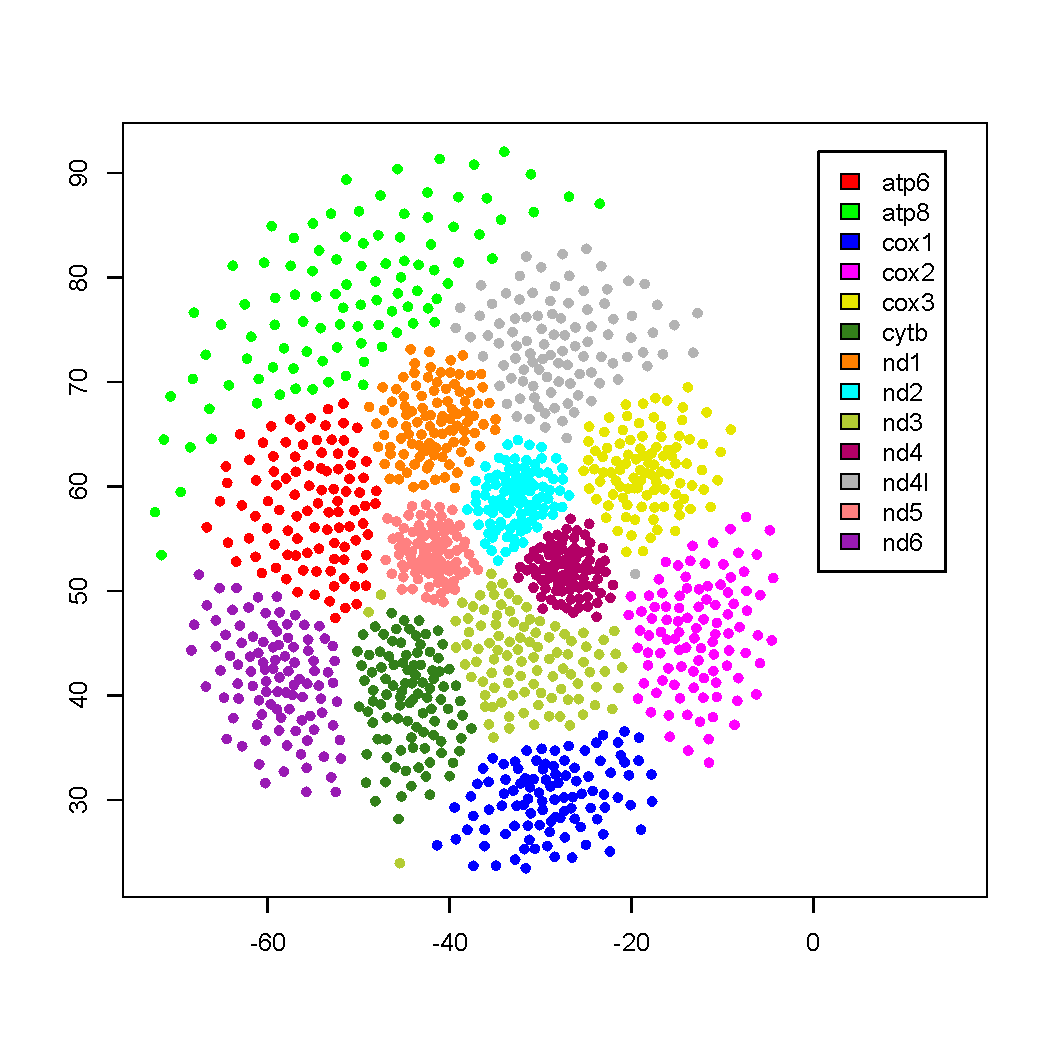
\includegraphics[scale=0.5]{imagesForManual/Figure1.pdf}
\caption{A $2-$dimensional representation of treespace generated by non-linear dimensionality reduction (NLDR) for a set of $1,300$ trees sampled from individual Bayesian analyses of $13$ mitochondrial protein-coding genes in squamates {\color{red}\bf (REFERENCE NEEDED: Castoe et al. 2009)}. Each point represents a tree sampled from the posterior distribution of one gene. One hundred trees were sampled from each posterior distribution. Points are colored by gene. Plot created using R.}\label{fig1}
\end{figure}
	
	
{\it Community Detection} -- When tree sets are summarized by condensing them into a single point estimate, one of the key pieces of lost information is whether distinct phylogenetic ``signals" exist in the set. Distinct signals can be created by a variety of biological processes like coalescence within a species, incomplete lineage sorting between species, horizontal gene transfer, hybridization, and migration. Artificial signals can also be created by systematic error during the process of phylogenetic inference. The process of detecting distinct signals in a tree set and assigning trees to one or more groups can be formalized in many different ways (e.g.,~\citep{GSAGD:2015,LM:2016}). TreeScaper uses a graph-theoretic approach known as community detection. Roughly speaking, communities are parts of a graph with dense, positive connections between nodes within a community and sparse or negative connections between nodes in different communities. By formalizing the problem of detecting distinct phylogenetic signals as a community detection problem, we can draw from a large body of existing work in graph theory. \\


TreeScaper can perform community detection on two distinct types of networks. In the first, nodes in the graph correspond to individual trees in the tree set and the edges between these nodes are weighted by the affinity between these trees (Fig.~\ref{fig2}). \\


Affinity can be calculated in different ways, but it broadly corresponds to the converse of distance -- a pair of trees separated by a small distance have high affinity, while a pair separated by a large distance have low affinity. Communities in these networks should intuitively correspond to sets of trees that are topologically similar to one another and topologically dissimilar to trees in other communities. Topological affinity networks have received some previous attention in attempts to define distinct phylogenetic signals {\color{red}\bf (REFERENCE NEEDED: Stockham et al. 2002)};~\citep{GSAGD:2015,LM:2016}. \\


The other type of network employed by TreeScaper uses nodes to represent individual bipartitions, with edge weights corresponding to the covariance in presence/absence of bipartition pairs across trees in the tree set (Fig. 3). When bipartitions are very common or very rare in the tree set, they tend to have weak covariances with all other bipartitions. However, if two bipartitions are present at intermediate frequencies and they are always found in the same trees or always found in different trees, they will have strong positive or strong negative covariances, respectively. Communities can be identified in bipartition covariance networks just like in topological affinity networks, with the distinction that bipartition covariance networks may contain negative edge weights. In this case, communities should consist of sets of bipartitions that tend to have strong positive covariances, while bipartitions in separate communities should tend to have strong negative covariances (Fig. 3). \\


\begin{figure}[thbp!]\centering
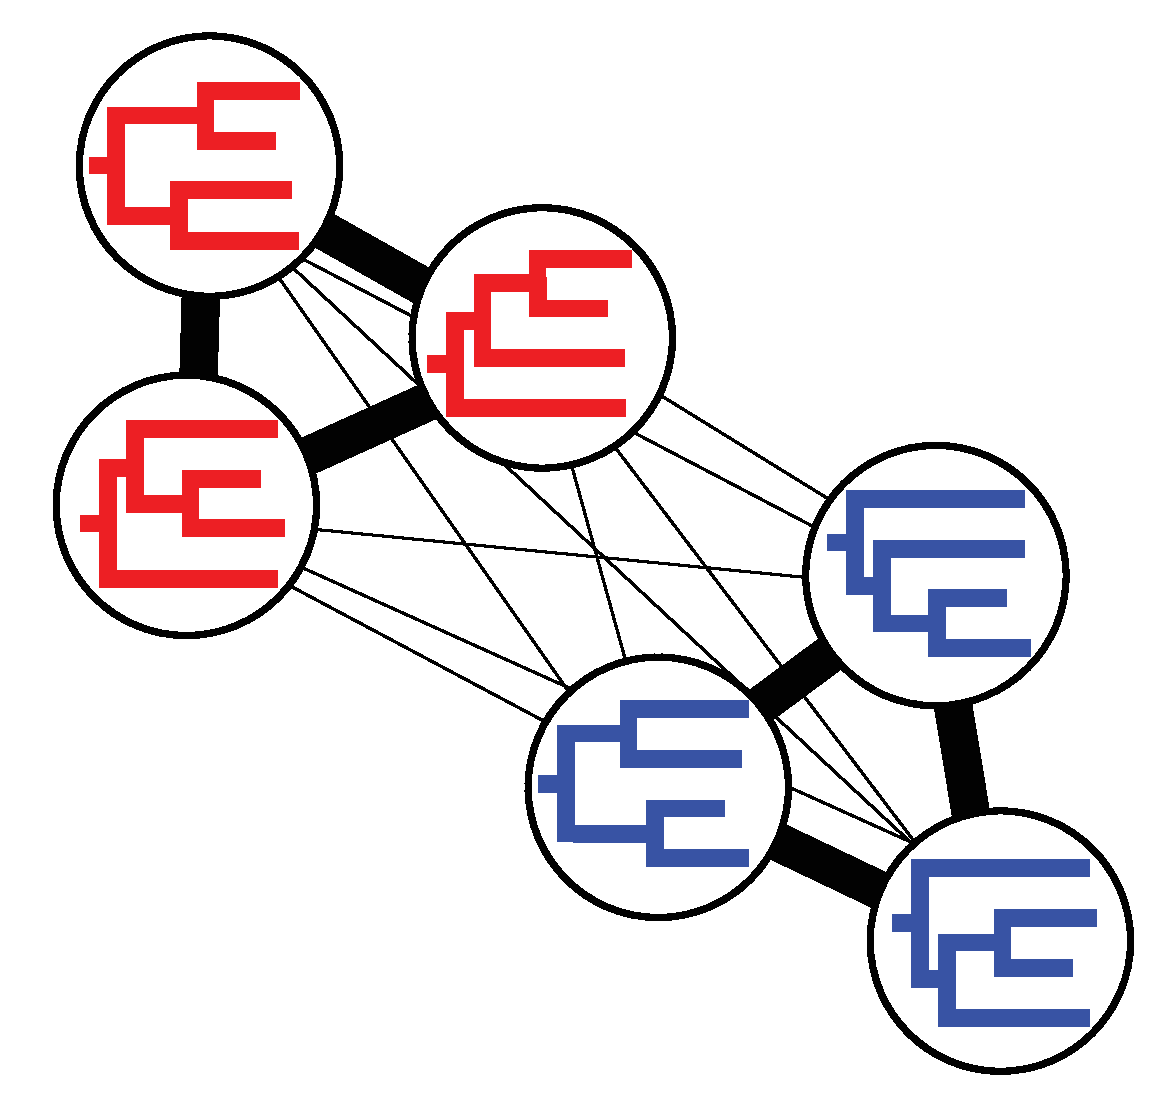
\includegraphics[scale=0.25]{imagesForManual/Figure2.pdf}
\caption{A cartoon topological affinity network. Circles are nodes in the network, each of which corresponds to one tree from a tree set. Edges represent the affinity (or similarity) between the trees, with thicker lines indicating greater affinity. Tree colors correspond to one intuitive definition of communities in this network.}\label{fig2}
\end{figure}


\begin{figure}[thbp!]\centering
\begin{subfigure}{0.4\textwidth}\centering
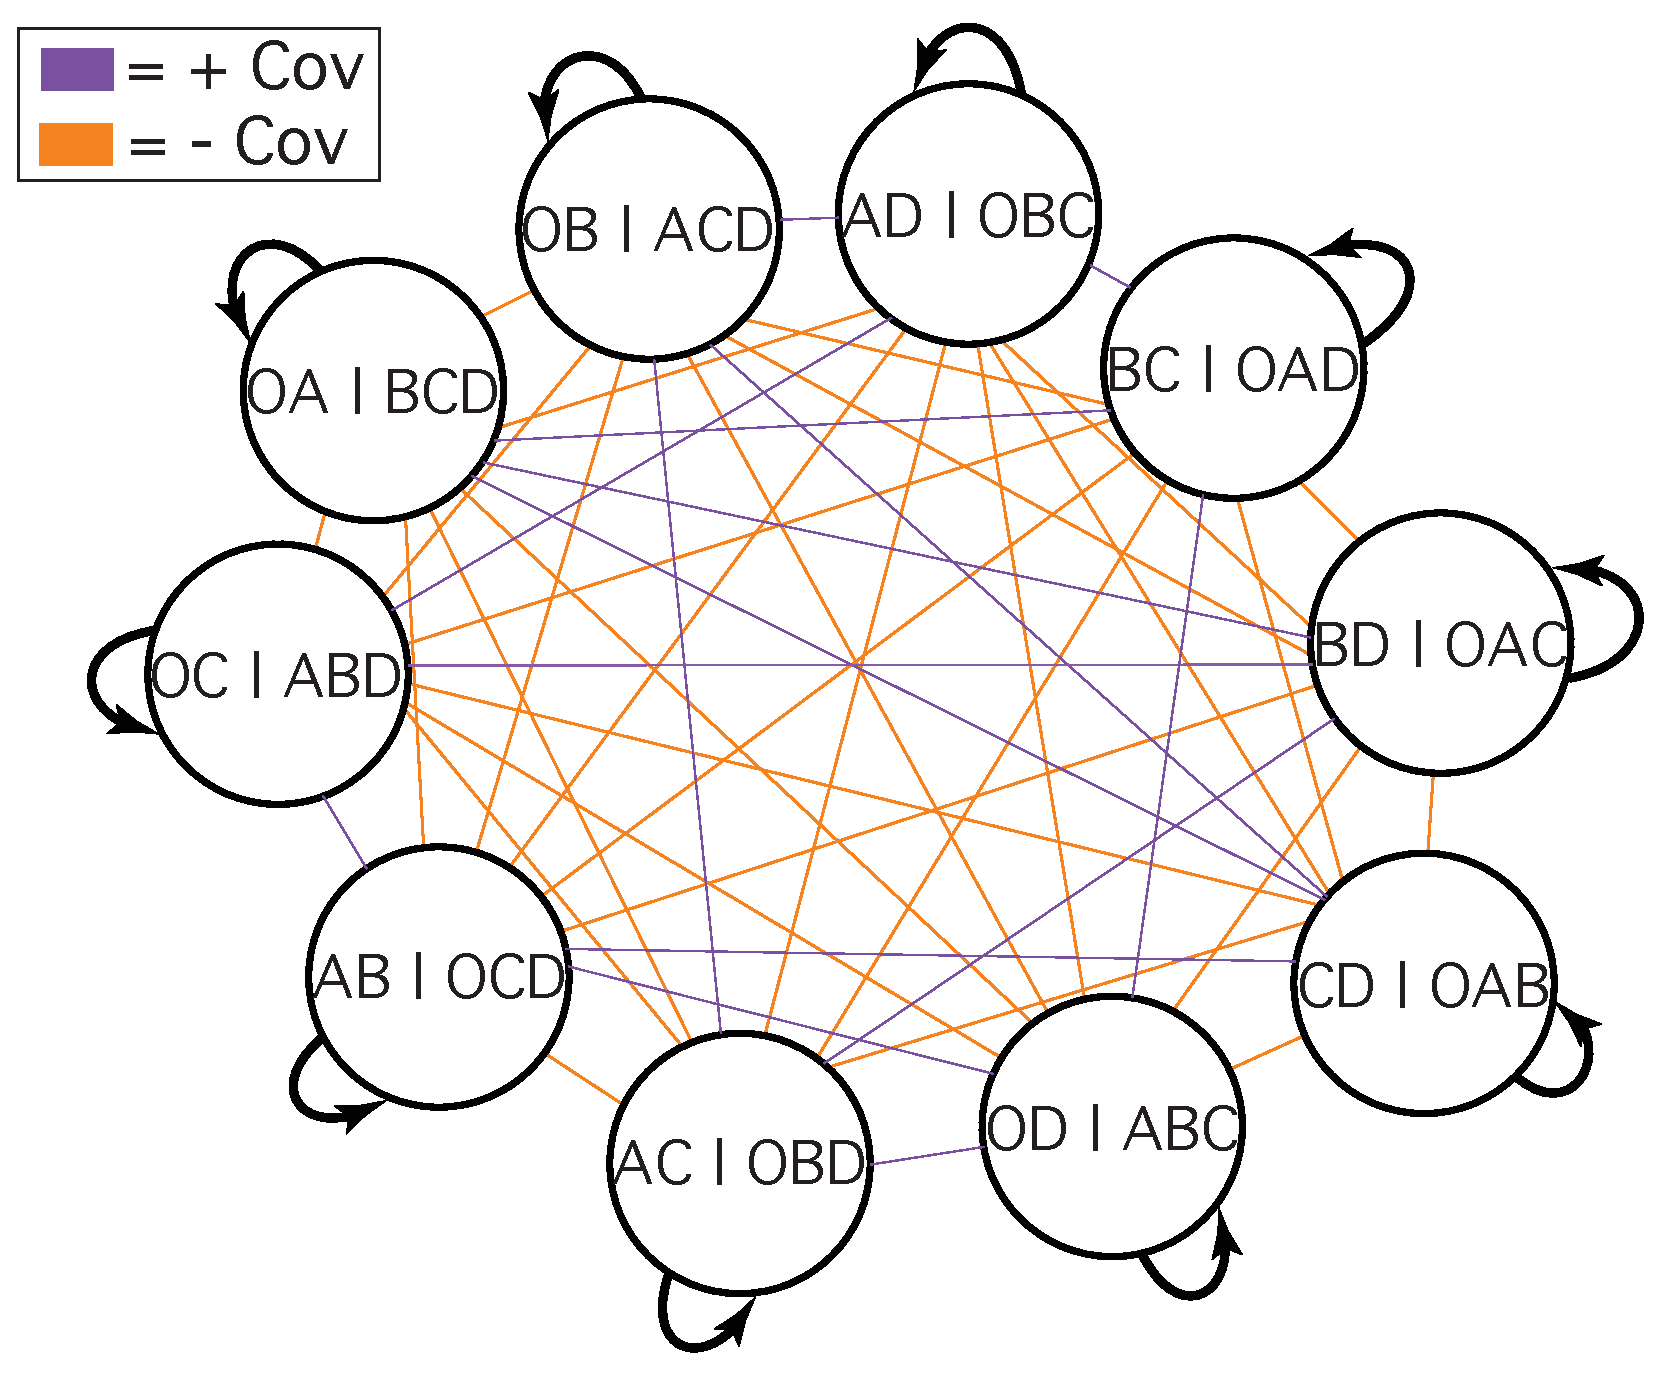
\includegraphics[scale=0.25]{imagesForManual/Figure3a.pdf}
\end{subfigure}
~ % add a little space
\begin{subfigure}{0.4\textwidth}\centering
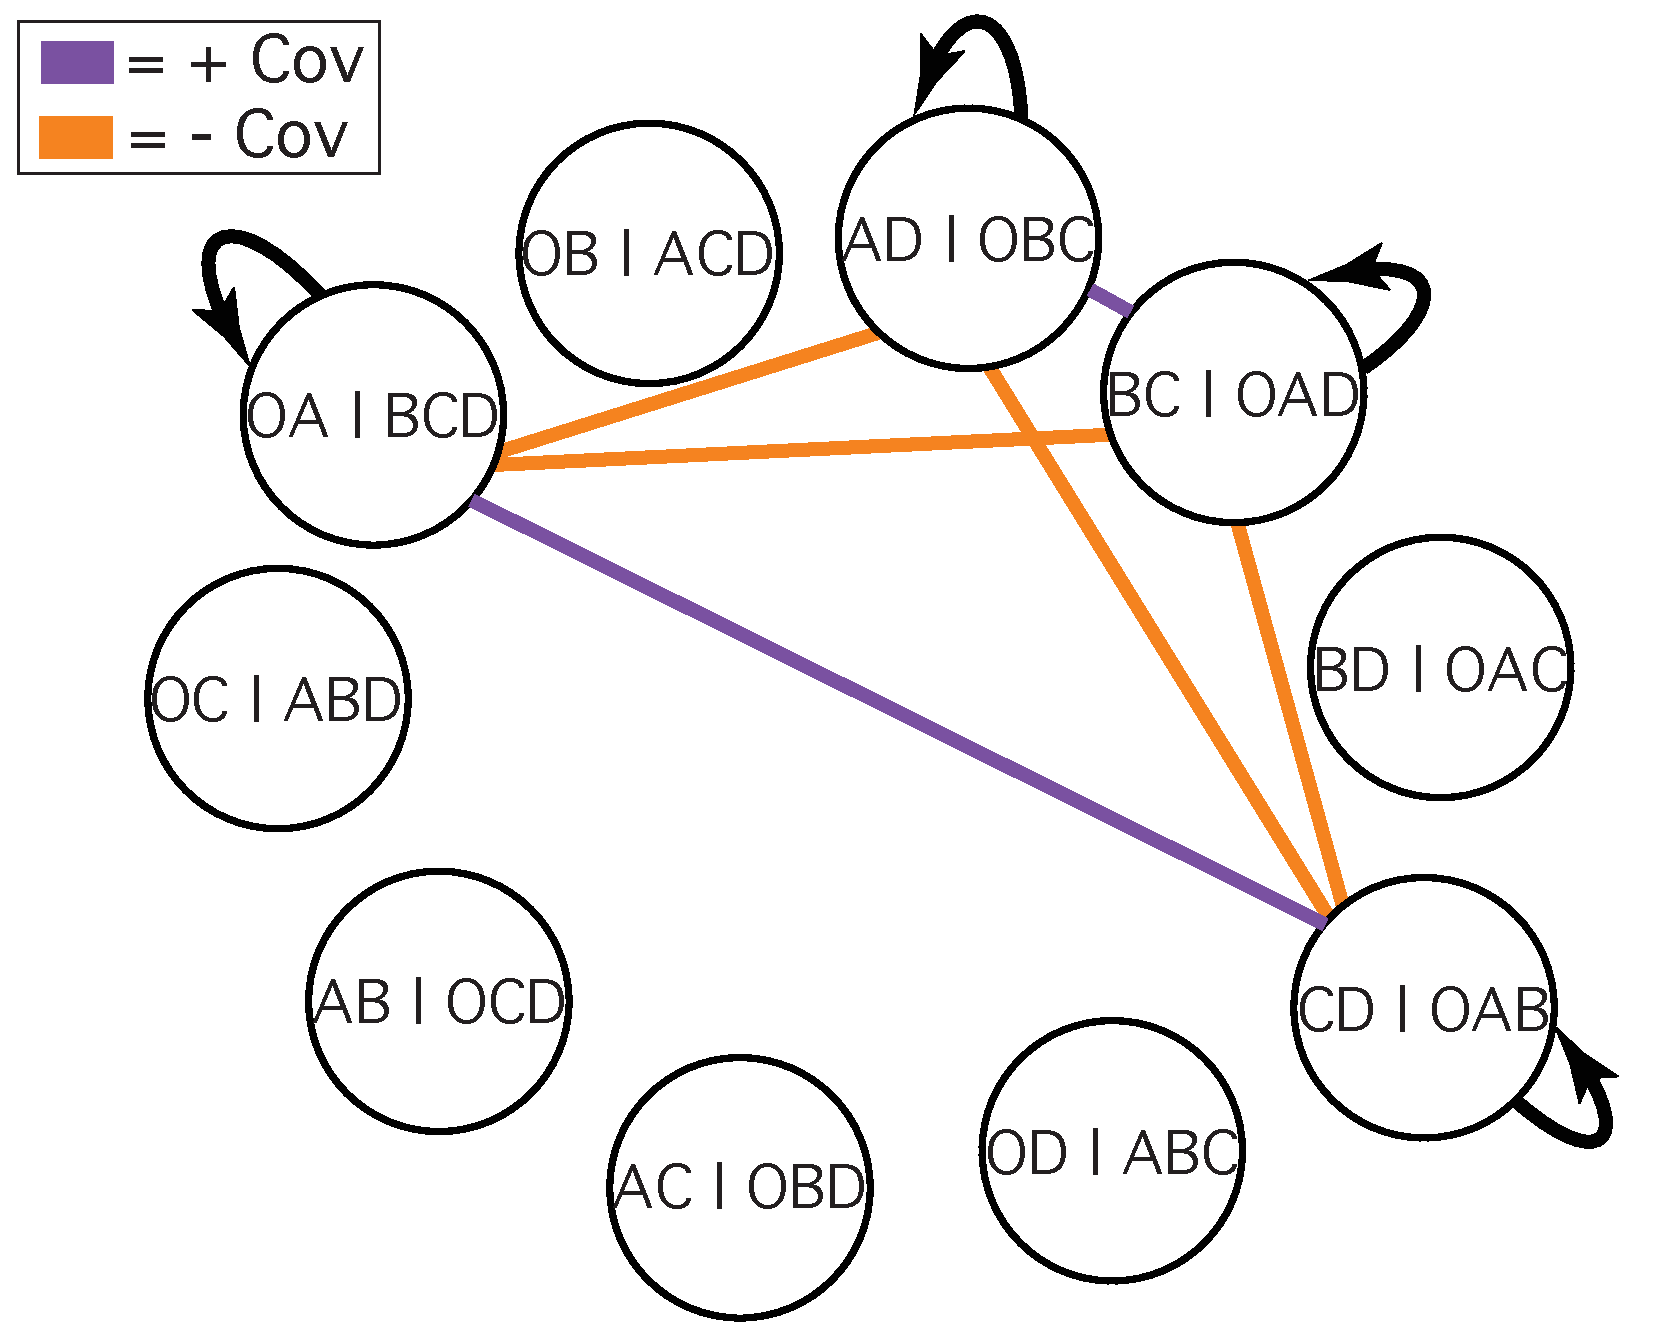
\includegraphics[scale=0.25]{imagesForManual/Figure3b.pdf}
\end{subfigure}

\caption{Two example bipartition covariance networks for sets of unrooted, $5-$taxon trees. The network on the left corresponds to a tree set with a uniform distribution of frequencies across all possible tree topologies. Some weak covariances exist in this network, because some pairs of bipartitions are mutually exclusive and are therefore found together less often than would be expected based on their frequencies alone. The network on the right corresponds to a tree set with only two topologies present at equal frequencies.}\label{fig3}
\end{figure}




%%%%%%%%%%%%%%%%%%%%%%%%%%%%%%%%%%%%%%%%%%%%%%%%%%%
% QUICKSTART TUTORIAL
%%%%%%%%%%%%%%%%%%%%%%%%%%%%%%%%%%%%%%%%%%%%%%%%%%%
\newpage
\section{QUICKSTART TUTORIAL}\label{sect:QuickstartTutorial}

%%%%%%%%%%%%%%%%%%%%%%%%%%%%%%%%%%%%%%%%%%%%%%%%%%%
% Getting Started
\subsection{Getting Started}\label{subsect:GettingStarted}

%%%%%%%%%%%%%%%%%%%%%%%%%%%%%%%%%%%%%%%%%%%%%%%%%%%
% Installation
\subsubsection{Installation}\label{subsubsect:Installation}

The Quickstart Tutorial uses a pre-compiled version of TreeScaper with a graphical user interface (GUI), which requires no special installation steps. Just download the appropriate version of the software from the TreeScaper website, open it, and get started. Pre-compiled versions of TreeScaper for Mac and Linux, as well as the files needed for this tutorial, are available here: \\

\noindent{\color{blue}\url{https://github.com/whuang08/TreeScaper/releases}} \\


\noindent {\bf\ul{Important Note:}} The default security settings on current versions of Mac OS X do not allow users to open applications that have been downloaded outside the App Store with a simple double-click. Instead, you will need to hold down control and single-click on the TreeScaper app, then select ``Open". When asked if you are sure, select ``Open" again.


%%%%%%%%%%%%%%%%%%%%%%%%%%%%%%%%%%%%%%%%%%%%%%%%%%%
% Example Tree Set
\subsubsection{Example Tree Set}\label{subsubsect:ExampleTreeSet}

The tree set that will be used throughout this tutorial is titled ``1000bp1L.nex".  The alignment used to generate this set of bootstrap trees was simulated such that half the sites were generated using one topology, while the other half were generated using another. ``guide\_tree1.pdf" and ``guide\_tree2.pdf" show the two topologies, corresponding to the first and second halves of the alignment, respectively.  Bipartitions that conflict between these topologies are in color.  A bootstrap analysis was then performed in Garli, to produce the $100$ trees in this tree set.  In this tutorial, we will analyze this tree set in TreeScaper to explore the two conflicting signals present in the data. \\


%%%%%%%%%%%%%%%%%%%%%%%%%%%%%%%%%%%%%%%%%%%%%%%%%%%
% Output
\subsubsection{Output}\label{subsubsect:Output}

At any point, you can use the data menu in the bottom left pane to see what data structures you have saved in memory.  Select any data structure and double click it to output or delete that data. Deleting data structures will allow you to control TreeScaper�s memory footprint. When outputting data structures, the name of the output file will be printed to the log. \\


%%%%%%%%%%%%%%%%%%%%%%%%%%%%%%%%%%%%%%%%%%%%%%%%%%%
% Saving Figures
\subsubsection{Saving Figures}\label{subsubsect:SavingFigures}

At this time, TreeScaper cannot natively save figures to file, so graphs and plots are most easily preserved through screen capture. On Macs, the Grab utility makes capturing and saving individual windows easy. For more customized versions of non-linear dimensionality reduction (NLDR) projections, users can read NLDR coordinates automatically written by TreeScaper into other software (e.g., R) and adjust settings as they see fit. \\


%%%%%%%%%%%%%%%%%%%%%%%%%%%%%%%%%%%%%%%%%%%%%%%%%%%
% Formatting Conventions
\subsubsection{Formatting Conventions}\label{subsubsect:Formatting}

Throughout this manual, we format the text differently when referring to different TreeScaper components for clarity. {\it Tabs and labels} are italicized, {\bf buttons} are bolded, ``options" are in quotes, and \ul{dropdown} menu options are underlined. \\


%%%%%%%%%%%%%%%%%%%%%%%%%%%%%%%%%%%%%%%%%%%%%%%%%%%
% Loading the Tree Set and Basic Computations
\subsection{Loading the Tree Set and Basic Computations}\label{subsubsect:LoadTreesBasicComp}

Starting off in {\it Trees and Bipartition Computation}, \ul{Load Tree Data} should already be selected. {\bf Browse} and select the tree file. Select ``weighted trees", but do not select ``rooted".  Click {\bf Load all Trees} to load the tree set into memory. \\


From the dropdown menu, now select \ul{Compute Bipartition Matrix}, then click the {\bf Compute Bipartition-Tree Matrix} button.  The log window will show a list of all the bipartitions in the tree set, along with their frequency. The data structure called ``Bipartition Matrix� now contains all trees and the bipartitions they contain, along with all the bipartition weights (i.e., branch lengths) for each tree. These data can be printed to a file in two different forms: as a list or as a matrix. In the list format, the first column indexes the unique bipartitions (which may be present in multiple trees), the second column indexes the trees in which those bipartitions were found, and the third column gives the bipartition weights. \\


Next, we�ll use the information in the bipartition-tree matrix to compute a consensus tree. To do so, select \ul{Compute Consensus Tree} from the dropdown menu. Leaving the default parameters alone, click {\bf Consensus Tree} and then {\bf Plot}. While examining the plot, you can zoom in and out by scrolling up or down. Holding down the option key while clicking and grabbing the plot will allow you to move the tree. You can see in the consensus tree that there is low bootstrap support ($< 0.7$) for several bipartitions in the consensus tree.   It is impossible to determine, from this consensus tree alone, whether the low support is due to a lack of phylogenetic signal or strong support for a few conflicting topologies. \\


%%%%%%%%%%%%%%%%%%%%%%%%%%%%%%%%%%%%%%%%%%%%%%%%%%%
% Visualizing Tree Space
\subsection{Visualizing Tree Space}\label{subsect:VisualizeTreeSpace}

First, to get an idea of what tree space looks like for this tree set, we will visualize it in 3D using a non-linear dimensionality reduction (NLDR) projection method.  In these projections, each point represents a tree in the tree set, and the distance between two points is an approximation of the actual tree-to-tree distance. From the main dropdown menu, select \ul{Load Distance/Coordinate Data or Compute Tree-to-Tree Distances}. In this case, we will calculate the tree-to-tree distances from scratch, but you could also load distances from file if they were calculated previously. If you plan on conducting many analyses with the same large tree set, storing and loading the tree distances will save considerable time. From the Method dropdown select \ul{Weighted Robinson Foulds}, then click {\bf Distance} to compute a matrix of pairwise distances between trees in your tree set. This matrix should appear as a new data structure in the bottom left pane. Also select \ul{Unweighted Robinson Foulds} and compute the distance. You will need to use this distance matrix later. We have now conducted all of the necessary preliminary calculations to conduct NLDR.\\


In the topmost tab menu, now select {\it NLDR and Dimension Estimation}. In the main dropdown menu under this tab, \ul{Nonlinear Dimension Reduction} should already be selected. Make sure that \ul{Weighted RF-distance} is selected in the {\it Distance} dropdown, with \ul{CCA} and \ul{Stochastic} selected in {\it Method and Algorithm} drop downs, respectively. Change {\it Dimension} to $3$. Make sure that \ul{Random} is selected in the {\it Initial Projection} dropdown. \\


Next, click the {\bf Plot Parameters} button.  A new dialogue box should appear.  \ul{Points} should be selected in the dialogue�s dropdown menu. Set the ``Number of Clusters" to $1$, then click {\bf OK}.  $1$ cluster should appear in the ``Cluster Index" section.  Check the ``Step Size" box.  Set the step size to $100$.  The single cluster should now include all $100$ trees in the tree set (with indices $0 - 99$). Under ``Other parameters" change ``point size" to $10$, then click {\bf Apply}, followed by {\bf Close}. \\


Now, click the {\bf Run NLDR} button.  Once the NLDR method is finished running, click {\bf Plot Result}.  A dialogue box with the plot of tree space should appear.  Click and drag to rotate the 3D plot. Scroll up and down to zoom in and out. Hold down Shift$+$R, select a small number of points ($1-5$), then click the {\bf Plot trees} button to examine each of these trees individually. By rotating the plot, you should see what looks like three distinct groups, or communities, of points.  The NLDR projection suggests that these communities have lower tree-to-tree distances between trees in the same community and larger distances between trees in different communities.  We will later confirm that the original tree-to-tree distances support these community designations by performing a community detection analysis on the tree set�s topological affinity network. After rotation, your NLDR plot should look something like Figure~\ref{fig4}.  In this diagram, trees are colored by affinity community, which we will find in the next step of the tutorial. TreeScaper�s NLDR plots (e.g., Fig.~\ref{fig4}) can be saved using screen capture (or the Grab utility on Mac). Customized versions of such plots can be created by reading raw NLDR coordinates into software such as R, which have more advanced plotting capabilities. See Section~\ref{subsubsect:CompBipartMatrix} for more details on NLDR plotting options and output files. \\

\begin{figure}[thbp!]\centering
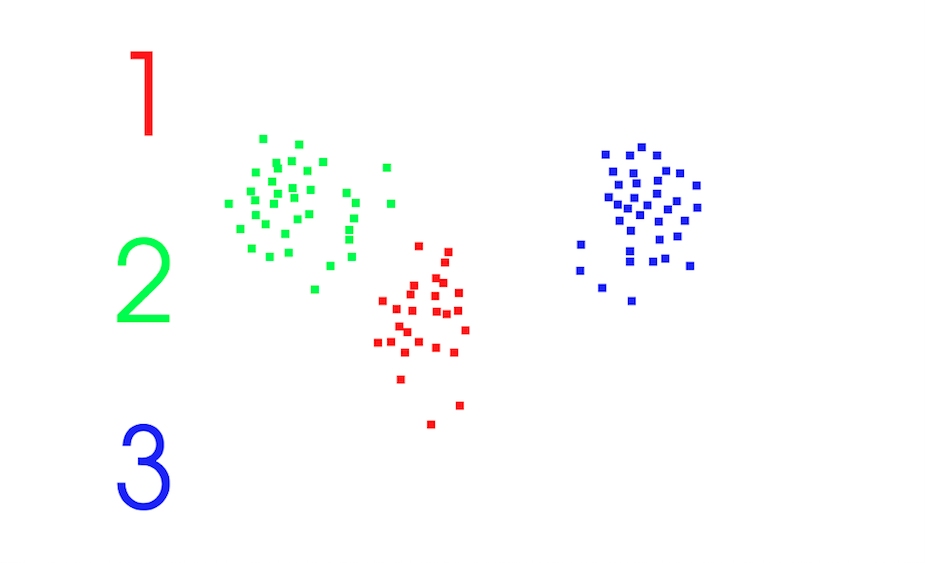
\includegraphics[scale=0.25]{imagesForManual/Figure4.png}
\caption{One rotation of the 3D NLDR projection outlined in the quickstart tutorial. Points are colored according to the output of topological affinity community detection analysis, which is described below.}\label{fig4}
\end{figure}


%%%%%%%%%%%%%%%%%%%%%%%%%%%%%%%%%%%%%%%%%%%%%%%%%%%
% Community Detection
\subsection{Community Detection}\label{subsect:CommunityDetection}

Before using community detection to identify distinct phylogenetic signals, we need
to construct networks using our tree set. We will then perform community detection on
these networks to identify distinct topological signals and the sets of bipartitions that strongly
conflict between them. As mentioned in the Introduction, TreeScaper uses two types of
networks: topological affinity and bipartition covariance networks. See above for more detail. \\

%%%%%%%%%%%%%%%%%%%%%%%%%%%%%%%%%%%%%%%%%%%%%%%%%%%
% Community Detection on a Topological Network
\subsubsection{Community Detection on a Topological Network}\label{subsubsect:CommunityDetectionTopologicalNetwork}

First, we will construct a topological affinity network, where nodes represent
individual trees in the tree set and edges between these nodes are weighted by the affinity
between the trees. Since affinities are the converse of distances, we need to convert our
previously calculated distances to affinities. In the topmost tab menu, go back to the {\it Trees
and Bipartition Computation} tab. Select \ul{Load/Convert Tree-to-Tree Distances to Affinities}
from the main dropdown menu in this tab. Select \ul{Unweighted RF-distance} from the {\it Distance
in Memory} dropdown. Make sure the {\it Affinity Type} is set to \ul{Reciprocal} then click {\bf Affinity}.
This will calculate the reciprocal of each distance in the distance matrix and use this as a
measure of affinity, or similarity, between the trees. \\


Now select the {\it Community Detection} tab at the top and \ul{Community Detection on
Affinities} from main dropdown menu. \ul{Affinity-URF} should be selected in the �``ffinity in
memory" dropdown. In the ``Model Type" dropdown select \ul{Constant Potts Model}, and in
``Find Plateaus" select ``Automatically". Click {\bf Community}. A variety of specific information
about the community detection analysis is printed to the log. For now, we will ignore most of
this information. The basic idea is to vary a tuning parameter (lambda) and see how the
inferred community structure changes. The preferred community structure is the one that is
most robust to changes in the tuning parameter. These naturally robust community
definitions are referred to as plateaus (which will make more sense in a moment). We prefer
the plateau with the largest ``lower bound length" value. This plateau should represent some
intrinsic community structure of the affinity matrix. \\


When community detection is finished, click {\bf Plot} to generate a figure showing how
various summaries of the inferred community structure change with varying values of 
lambda. For now, we will focus on the ``Labels for Communities" line and look for the largest
flat region (a plateau!) where the community labels remain stable as lambda varies. Note that
plateaus frequently occur on the left and right ends of these plots, but they represent trivial
community structures where all nodes are placed in a single community (the left end) or
every node is assigned to its own unique community (the right end). In this example, the
plateau of interest occurs when lambda is between $0.6$ and $0.9$. See Section~\ref{subsect:CommunityDetectionMenu} of this manual
and the Appendix~\ref{appendix:CDModels} for more details on why TreeScaper uses this definition of intrinsic community structure. Pick a $\lambda+$ value in the range of $\lambda+$ values corresponding to the plateau ($0.7$, for example). Returning to the main window, select ``Manually" for the ``Find Plateaus" option. Set both the ``From" and ``To" values to the chosen $\lambda+$ value. Click {\bf Community}. The plateau community structure will be printed to the log pane. For now, we are primarily interested in which trees (i.e., nodes in the network) are assigned to each community. \\


Using the indices of trees assigned to different communities, you can create
community-specific consensus trees or color points by community assignment in NLDR
plots. Copy the node indices corresponding to a community (e.g., those numbers that follow
``Community $1$ includes nodes:" in the log) and create a separate index file for each
community that has each number on its own line (see the format of ``example\_index\_aff1.txt"
for each affinity community or use the pre-made files, ``example\_index\_aff1-3.txt"). Go back
to \ul{Compute Consensus Tree} under {\it Trees and Bipartition Computation}, select �index file� in
``Considered Trees". Then, load an index file for the community of your choice. Click
{\bf Consensus Tree}, and then {\bf Plot}. The consensus tree for each affinity community should
provide a sense for its dominant phylogenetic signal. The files,
``AffinityConsensusCommunity1-3.pdf", show the affinity community consensus trees,
although the ordering of the three trees is arbitrary. Conflicting bipartitions from the two
topologies used to simulate the data are in color. \\


To color points in an NLDR plot by community, create a comma-separated list of the
indices for that community. Return to the {\it NLDR and Dimension Estimation} tab and click the
{\bf Plot Parameters} button. Change the number of clusters to $3$. In the box for each cluster
under {\it Cluster Index} paste the comma-separated list of indices for each community. Press Tab
after pasting each set of values, then click {\bf Apply} and {\bf Close}. Once back at the NLDR menu,
click {\bf Plot result}. The new plot should have the same structure as the previous NLDR plot,
but with points colored as in Fig.~\ref{fig4}. \\


%%%%%%%%%%%%%%%%%%%%%%%%%%%%%%%%%%%%%%%%%%%%%%%%%%%
% Community Detection on a Bipartition-Covariance Network
\subsubsection{Community Detection on a Bipartition-Covariance Network}\label{subsubsect:CommunityDetectionBipartCovNetwork}

Next, we will construct a bipartition covariance network. Go back through the steps
of Section~\ref{subsubsect:LoadTreesBasicComp} to reload the tree set, with one important difference: {\it do not select the ``weighted trees" option}. You should never use weighted trees to compute a covariance matrix, as the computed values will correspond to covariances in branch lengths rather than bipartition presence/absence. When you read the tree set back in without weights, all of the previous
data structures will automatically be erased. As	before, select \ul{Compute Bipartition Matrix}
from	the main dropdown menu and	click	{\bf Compute Bipartition-Tree Matrix}. \\


Now, select \ul{Load/Compute Bipartition Covariances} from the main dropdown, then
click {\bf Covariance using Bipartition-Tree Matrix}. Alternatively, you have the option to load a
previously computed covariance matrix at this stage. Once the covariance matrix has been
created, select the {\it Community Detection} tab at the top and choose \ul{Community Detection on
Covariances}. The \ul{Covariance Matrix} option should now appear in the ``Covariance in
Memory" dropdown. Set the ``High Freq" to $0.95$ and the ``Low Freq" to $0.05$. These settings
will filter out high and low frequency bipartitions, because they are very difficult to assign to
particular communities. In the ``Model Type" dropdown select \ul{Constant Potts Model}, and
for ``Find Plateaus" select ``Automatically". Click {\bf Community}. The lambda values used and
the largest plateaus are output to the log. The largest plateau is the plateau with the largest
``lower bound length" values. This plateau indicates the intrinsic community structure of the
covariance matrix. \\


When community detection is finished, click {\bf Plot} (Fig.~\ref{fig5}). As with community
detection for affinity networks, this plot will give you an intuitive sense for the most stable
community structure -- the largest plateau on the ``Labels for communities" line. Also as with
affinity networks, plateaus frequently occur on the left and right ends of these plots, but they
represent trivial community structures where all nodes are placed in a single community (the
left end) or every node is assigned to its own unique community (the right end). For this
example, there is $1$ community in the left trivial plateau and $10$ communities in the right
trivial plateau.\\ 


\begin{figure}[thbp!]\centering
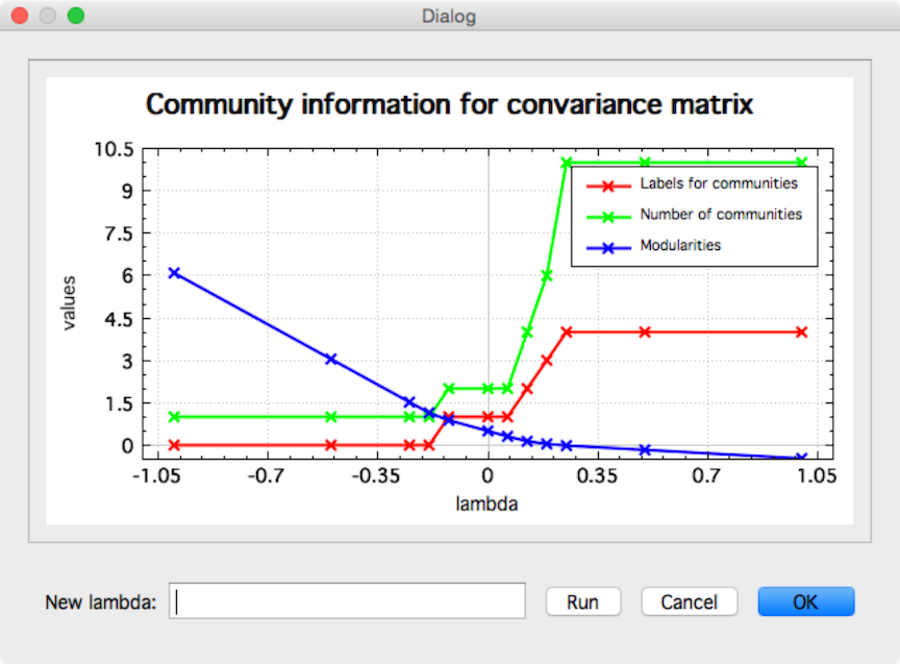
\includegraphics[scale=0.7]{imagesForManual/Figure5.pdf}
\caption{Example output from automatic community detection on the bipartition
covariance network discussed in the tutorial. Note the trivial community structures
represented by the plateaus at $1$ and $10$ communities.}\label{fig5}
\end{figure}


Pick a $\lambda+$ value in the range of $\lambda+$ values for the largest non-trivial plateau ($0$, for
instance). In {\it Find Plateaus} select ``Manually". In {\it $\lambda1$ Fixed}, select $\lambda^{-}$ and set the value to $0$. Set both the {\it From} and {\it To} values to be the chosen $\lambda^{+}$ value. Click {\bf Community}. The plateau community structure will be printed to the log. While TreeScaper does not have built-in functionality to visualize bipartition networks and communities, you can examine the bipartition matrix itself to see which bipartitions are assigned to each community. See the
``Compute Bipartition-Tree Matrix" menu in Section~\ref{subsubsect:CommunityDetectionBipartCovMenu} for an explanation of how to read
the bipartition matrix output. \\


The file ``1000bp1L\_comKey.out" shows the bipartitions assigned to each community,
along with their frequencies. Recall that the dataset used to generate this tree set was
simulated such that half the sites evolved on one topology and the other half evolved along
another (see ``guide\_tree1.pdf" and ``guide\_tree2.pdf", respectively, where conflicting
bipartitions are shown in color). The file ``1000bp1LcovarianceNetwork.pdf" contains a
schematic of the bipartition-covariance network. Node numbers correspond to the numbered
bipartitions in the guide trees. Blue and green edges indicate positive and negative
covariances between bipartitions, respectively. Line weights correspond to the magnitude of
the covariances. Colored circles circumscribe the nodes assigned to each of the detected
communities. Each community contains the conflicting bipartitions from one of the two
topologies used in the simulation. Thus, we have identified the conflicting bipartitions that
define the two distinct topological signals underlying the sites in this alignment. In the
affinity network, we also identified both of the original tree topologies and a third topology
that seems to arise when bootstrapped alignments contain balanced mixtures of sites of the
two types. \\


%%%%%%%%%%%%%%%%%%%%%%%%%%%%%%%%%%%%%%%%%%%%%%%%%%%
% INSTALLATION
%%%%%%%%%%%%%%%%%%%%%%%%%%%%%%%%%%%%%%%%%%%%%%%%%%%
\newpage
\section{INSTALLATION}\label{sect:Installation}

Executable versions of TreeScaper for Mac or Linux can be downloaded from \\

\noindent{\color{blue}\url{https://github.com/whuang08/TreeScaper/releases}} \\


Also available as separate downloads are files needed for the Quickstart tutorial at the
beginning of this manual and the source code corresponding to the most recent release of
TreeScaper. The most current (although not officially released) code is available from the
corresponding GitHub repository: \\

\noindent{\color{blue}\url{https://github.com/whuang08/TreeScaper}}\\


The graphical, pre-compiled version of TreeScaper can be started by simply doubleclicking (the name will either be ``TreeScaper" or ``TreeScaper.app").\\


\noindent \ul{\bf One Important Note for Macs:} The default security settings on current versions of Mac OSX do not allow users to open applications that have been downloaded outside the App Store
with a simple double-click. Instead, you will need to hold down control and single-click on
the TreeScaper app, then select ``Open". When asked if you are sure, select ``Open" again. \\


Command-line versions of TreeScaper can be generated by following these instructions:
\begin{enumerate}[(1)]
\item Download ``clapack-3.2.1-CMAKE.tgz" from {\color{blue}\url{http://www.netlib.org/clapack/}} and
unpack the archive.

\item If using a Mac, open the ``makefile.inc.example" file in the clapack folder and change
the platform from ``\_LINUX" to ``\_MAC". If using Linux, leave the platform as is.
Next, rename the file to ``makefile.inc".

\item Open a terminal, change directories (cd) into the clapack folder, then type ``make" to
compile cmake.

\item Open the Makefile in the folder containing TreeScaper code and simply replace
``$<$PATH\_TO\_CLAPACK$>$" with the path to your clapack cmake installation.

\item Finally, open the wdef.h file in the TreeScaper folder. On the 2$^{nd}$ \#define line, replace
\_MAC with COMMAND\_LINE\_VERSION

\item Now, in Terminal type ``make" to compile Treescaper. \\
\end{enumerate}



%%%%%%%%%%%%%%%%%%%%%%%%%%%%%%%%%%%%%%%%%%%%%%%%%%%
% TREESCAPER GUI MENUS
%%%%%%%%%%%%%%%%%%%%%%%%%%%%%%%%%%%%%%%%%%%%%%%%%%%
\newpage
\section{TREESCAPER GUI MENUS}\label{sect:TreeScaperGuiMenus}

TreeScaper�s windows are arranged in a series of tabs, organized by the different types
of analyses that TreeScaper can perform. Each tab contains a header at the top of its window
that specifies its features. Every tab also contains a data window at the bottom left which
shows the data structures currently available in memory. Each data structure may be deleted
or output to file by double clicking and selecting the relevant option. The TreeScaper log is
visible on the right side no matter which tab is selected. The log can be reset by clicking {\bf Clear
log}. All the example files mentioned below are included in the tutorial files available for
download from the TreeScaper website. \\


%%%%%%%%%%%%%%%%%%%%%%%%%%%%%%%%%%%%%%%%%%%%%%%%%%%
% Trees and Bipartition Computation
\subsection{Trees and Bipartition Computation}\label{subsect:TreeBipartComp}


%%%%%%%%%%%%%%%%%%%%%%%%%%%%%%%%%%%%%%%%%%%%%%%%%%%
% Load Tree Data
\subsubsection{Load Tree Data}\label{subsubsect:LoadTreeData}

\begin{figure}[thbp!]\centering
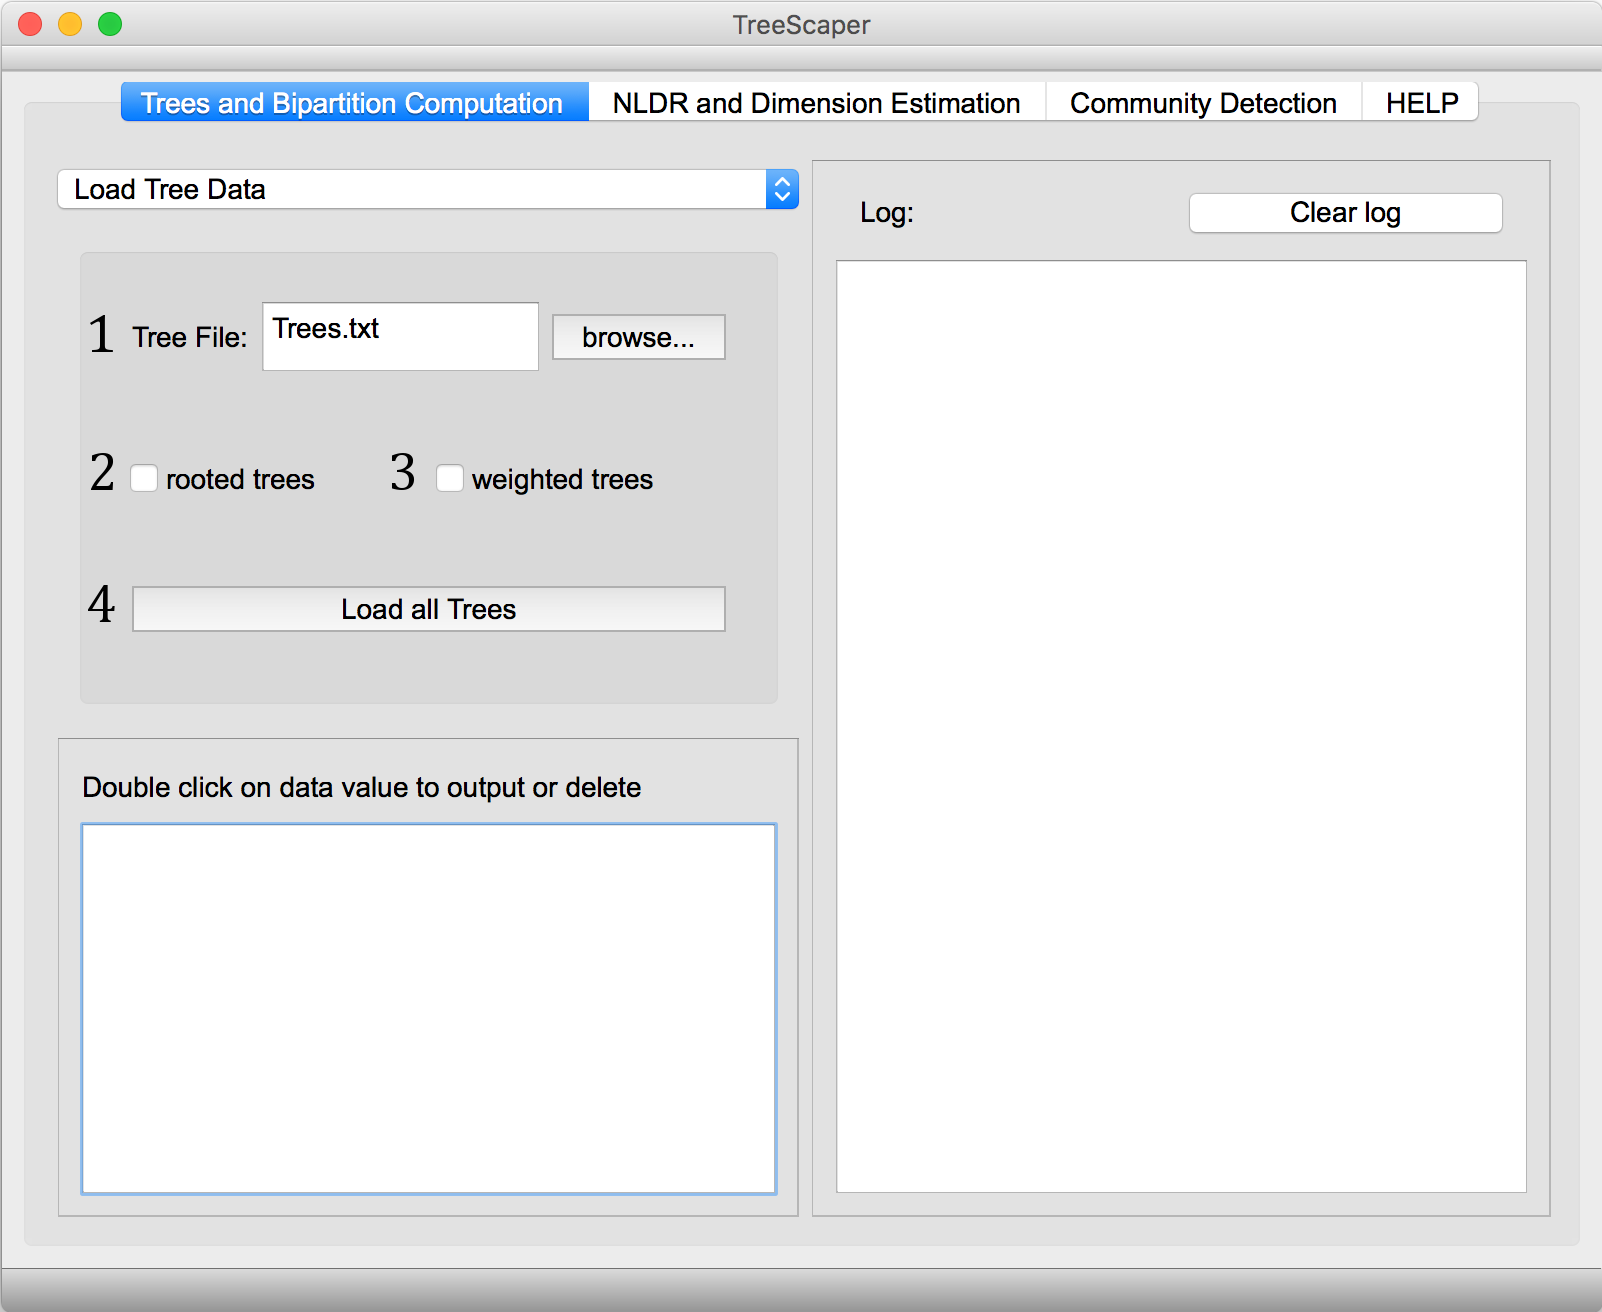
\includegraphics[scale=0.4]{imagesForManual/Figure6_6_1_1.png}
%\caption{}\label{fig6}
\end{figure}

\begin{enumerate}[{\bf 1-}]
\item {\bf [Tree File]} -- Select the location of the tree set. The tree set file needs to formatted as closely
to ``1000bp1L.nex" as possible. Make sure that there is a ``translate" section in the header of
the file. Comments in brackets are fine.

\item {\bf [rooted trees]} -- A checked box means the tree set contains rooted trees. An unchecked box
means the tree set contains unrooted trees.

\item {\bf [weighted trees]} -- A checked box means the tree set contains trees with branch lengths. An
unchecked box means the tree set contains trees without branch lengths.

\item {\bf [Load all Trees]} -- Load the tree set from the file specified in ``Tree File" into memory.
\end{enumerate}


%%%%%%%%%%%%%%%%%%%%%%%%%%%%%%%%%%%%%%%%%%%%%%%%%%%
% Compute Bipartition Matrix
\newpage
\subsubsection{Compute Bipartition Matrix}\label{subsubsect:CompBipartMatrix}

\begin{figure}[thbp!]\centering
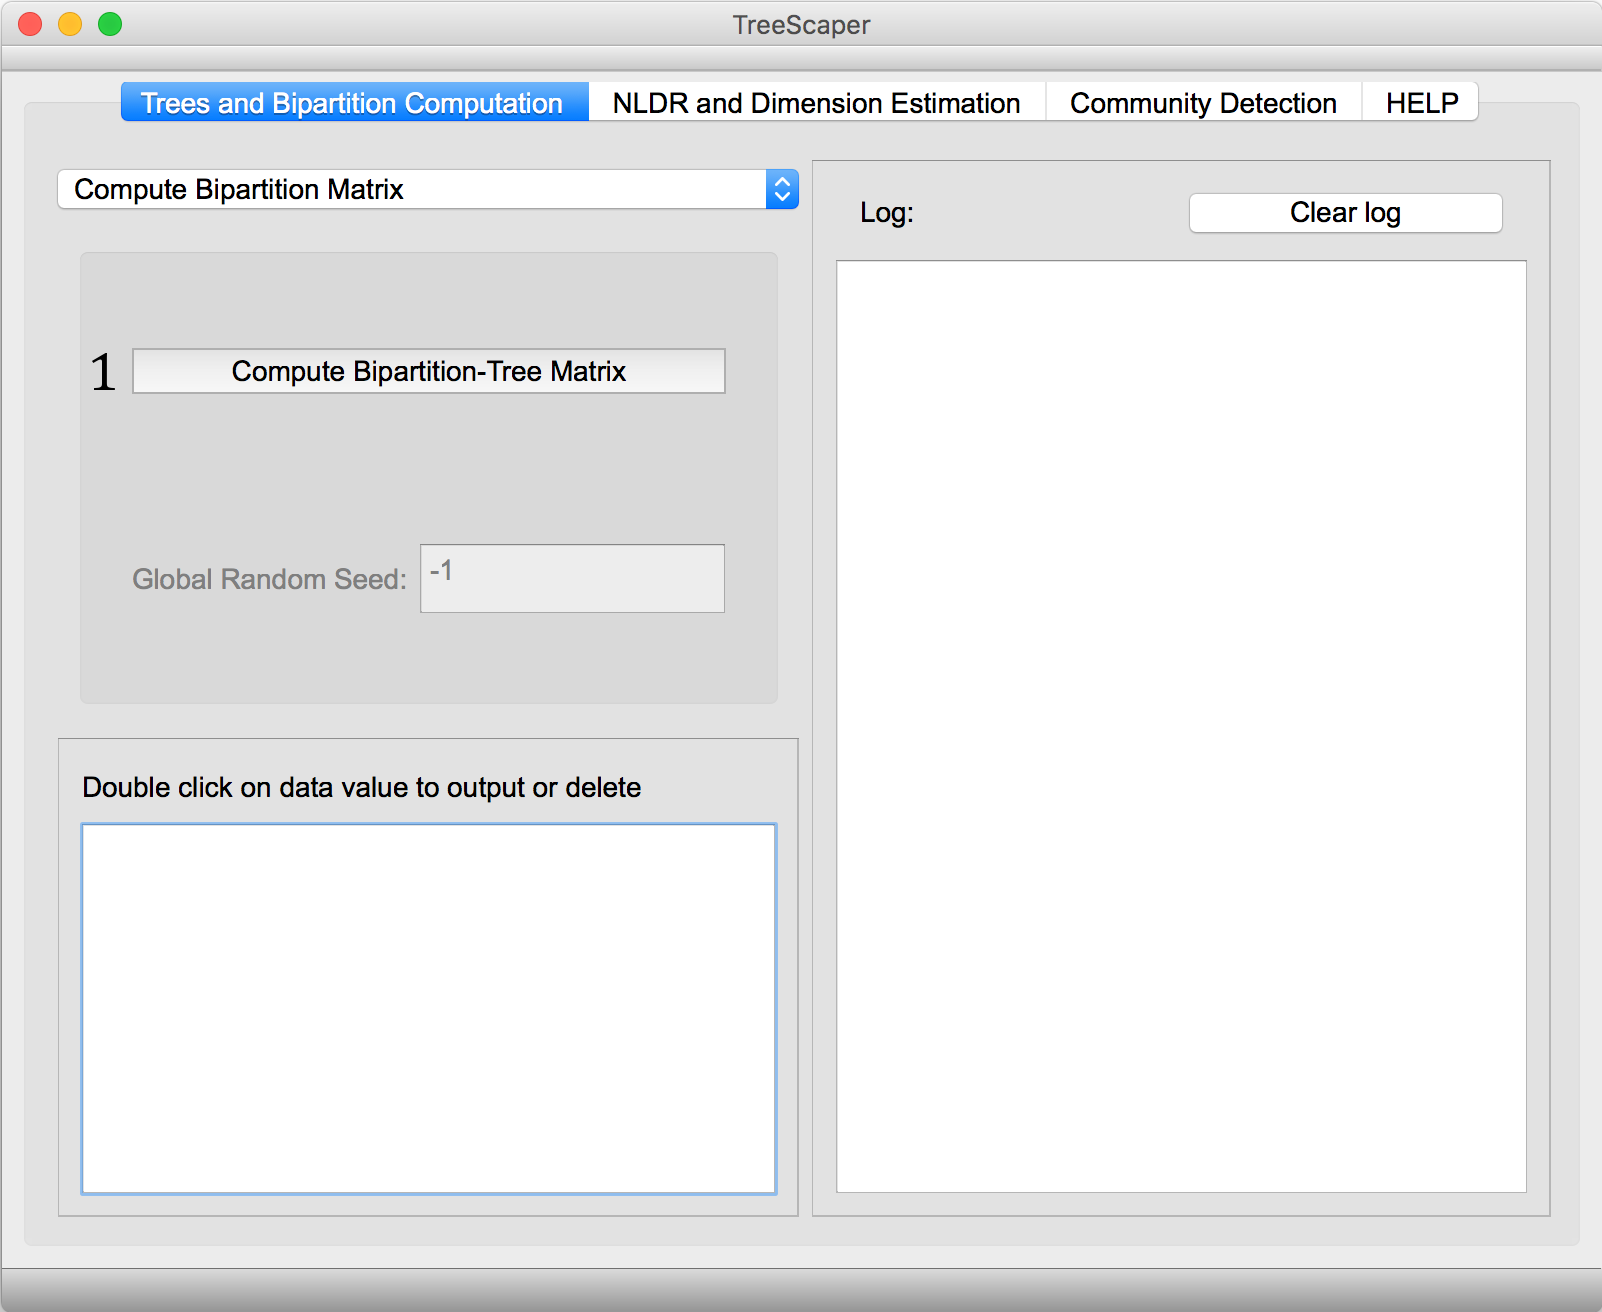
\includegraphics[scale=0.4]{imagesForManual/Figure7_6_1_2.png}
%\caption{}\label{fig7}
\end{figure}

\begin{enumerate}[{\bf 1-}]
\item {\bf [Computed Bipartition-Tree Matrix]} -- Creates a list of all the bipartitions in the tree set,
along with their number of occurrences, as well as a matrix of bipartition presence/absence
across trees. The bipartitions are specified using a binary notation, where all taxa on each side
of the bipartition have the same digit ($0$ or $1$). The order of binary digits corresponds to the
numbering of the taxa in the output taxa list. For example, the fifth digit in a bipartition�s
notation would correspond to the fifth taxon. For a six-taxon case (taxa A-F), $110000$ would
indicate a bipartition separating taxa A and B from taxa C-F.
\end{enumerate}


%%%%%%%%%%%%%%%%%%%%%%%%%%%%%%%%%%%%%%%%%%%%%%%%%%%
% Load/Compute Bipartition Covariances
\newpage
\subsubsection{Load/Compute Bipartition Covariances}\label{subsubsect:LoadCompBipartCov}

\begin{figure}[thbp!]\centering
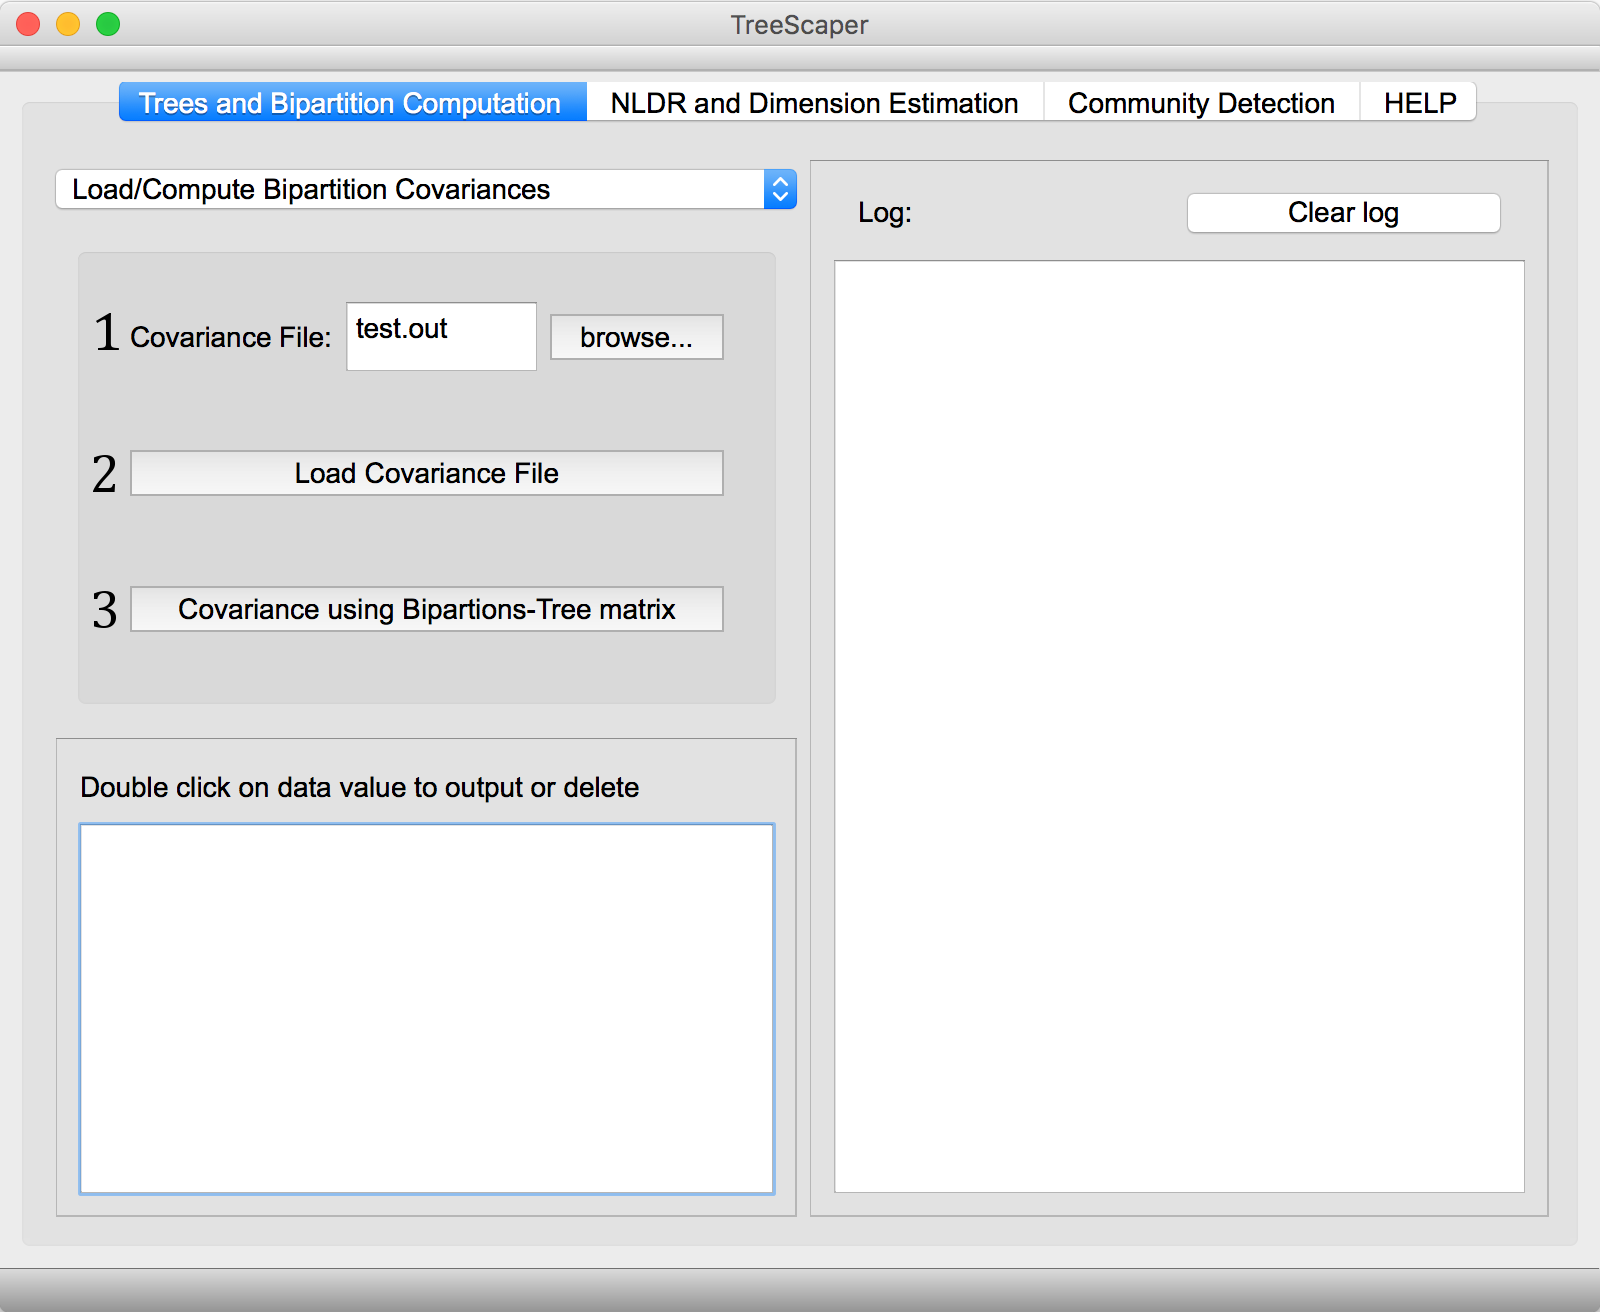
\includegraphics[scale=0.4]{imagesForManual/Figure8_6_1_3.png}
%\caption{}\label{fig8}
\end{figure}

\begin{enumerate}[{\bf 1-}]
\item {\bf [Covariance File]} --  Select the location of a covariance matrix (if previously computed).
The matrix needs to be similar to the format of ``1000bp1L\_Covariance Matrix.out" and will
usually correspond to the output of a prior TreeScaper analysis. This is a lower triangle
matrix where the rows and columns are labeled according to the bipartitions in the tree set,
and cells give covariances in bipartition presence/absence across trees.

\item {\bf [Load Covariance File]} -- Load covariance matrix into memory (if selected).

\item {\bf [Covariance using Bipartition-Tree matrix]} -- Use the bipartition-tree matrix stored in
memory to compute a covariance matrix. In general, DO NOT use weighted trees to compute
a covariance matrix, because the computed values will correspond to covariances in branch
lengths rather than bipartition presence/absence.
\end{enumerate}

%%%%%%%%%%%%%%%%%%%%%%%%%%%%%%%%%%%%%%%%%%%%%%%%%%%
% Compute Consensus Tree
\newpage
\subsubsection{Compute Consensus Tree}\label{subsubsect:CompConsensusTree}

\begin{figure}[thbp!]\centering
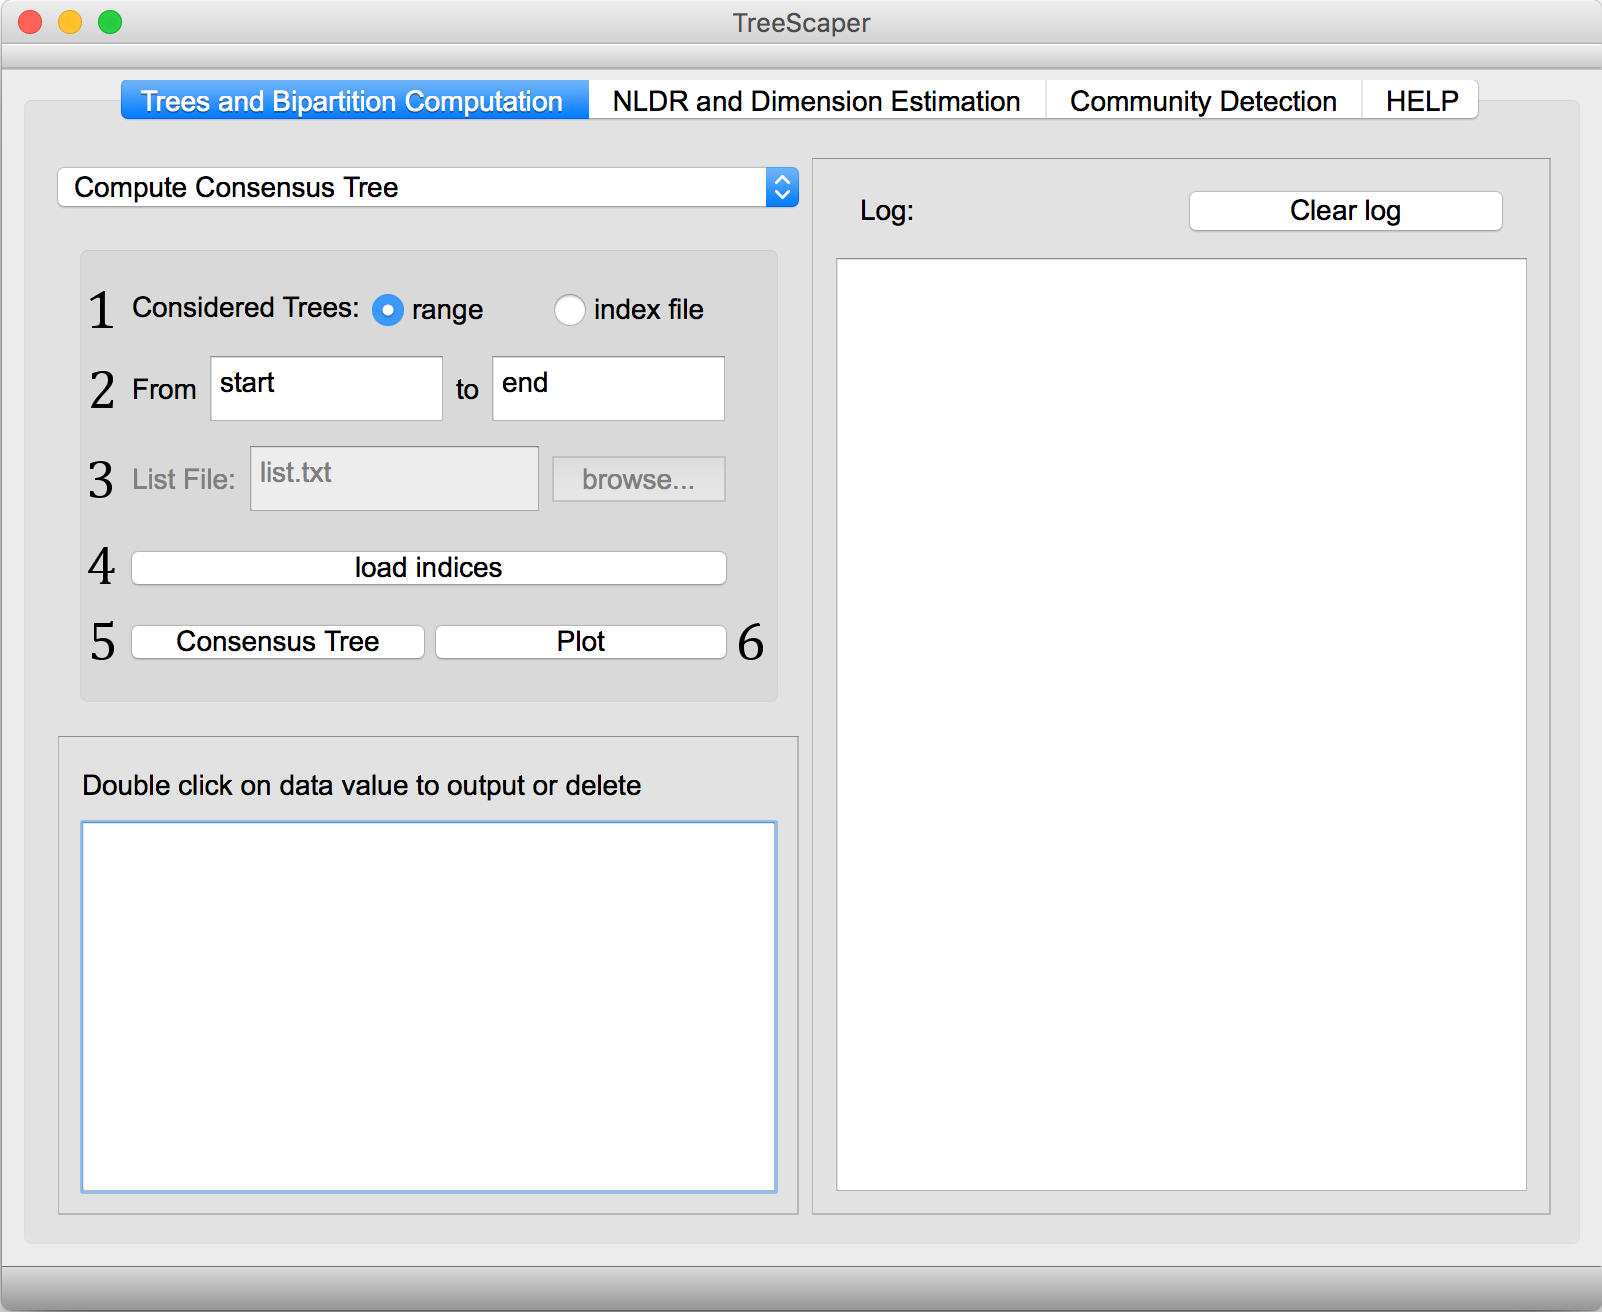
\includegraphics[scale=0.4]{imagesForManual/Figure9_6_1_4.png}
%\caption{}\label{fig9}
\end{figure}

\begin{enumerate}[{\bf 1-}]
\item {\bf [Considered Trees]} --  Select the trees to be considered when computing a consensus tree. A
manually defined range of tree indices can be provided by selecting ``range", or a series of
indices can be specified in a list contained in a file by selecting ``index file".

\item {\bf [range]} -- The indices of a range of trees to consider when calculating a consensus tree.
These values are needed if ``range" is specified for the ``Considered Trees". By default, the
range is the whole tree set, from ``start" to ``end".

\item {\bf [List file]} -- Considers trees listed in an index file. Specify the location of the file in ``List
File". The index file must be in the format of ``indices.out", with one tree index per line.

\item {\bf [load indices]} -- Loads the index (i.e., list) file into memory, if ``index file" is selected for
``Considered Trees".

\item {\bf [Consensus Tree]} -- Compute the consensus tree of selected trees.

\item {\bf [Plot]} -- Plot the consensus tree in a separate window. Use the mouse scroll bar to zoom.
COMMAND$+$click$+$drag to move the tree and zoom in at the desired location.
\end{enumerate}

%%%%%%%%%%%%%%%%%%%%%%%%%%%%%%%%%%%%%%%%%%%%%%%%%%%
% Load Distance/Coordinate Data or Compute Tree-to-Tree Distances
\newpage
\subsubsection{Load Distance/Coordinate Data or Compute Tree-to-Tree Distances}\label{subsubsect:LoadCompDist}

\begin{figure}[thbp!]\centering
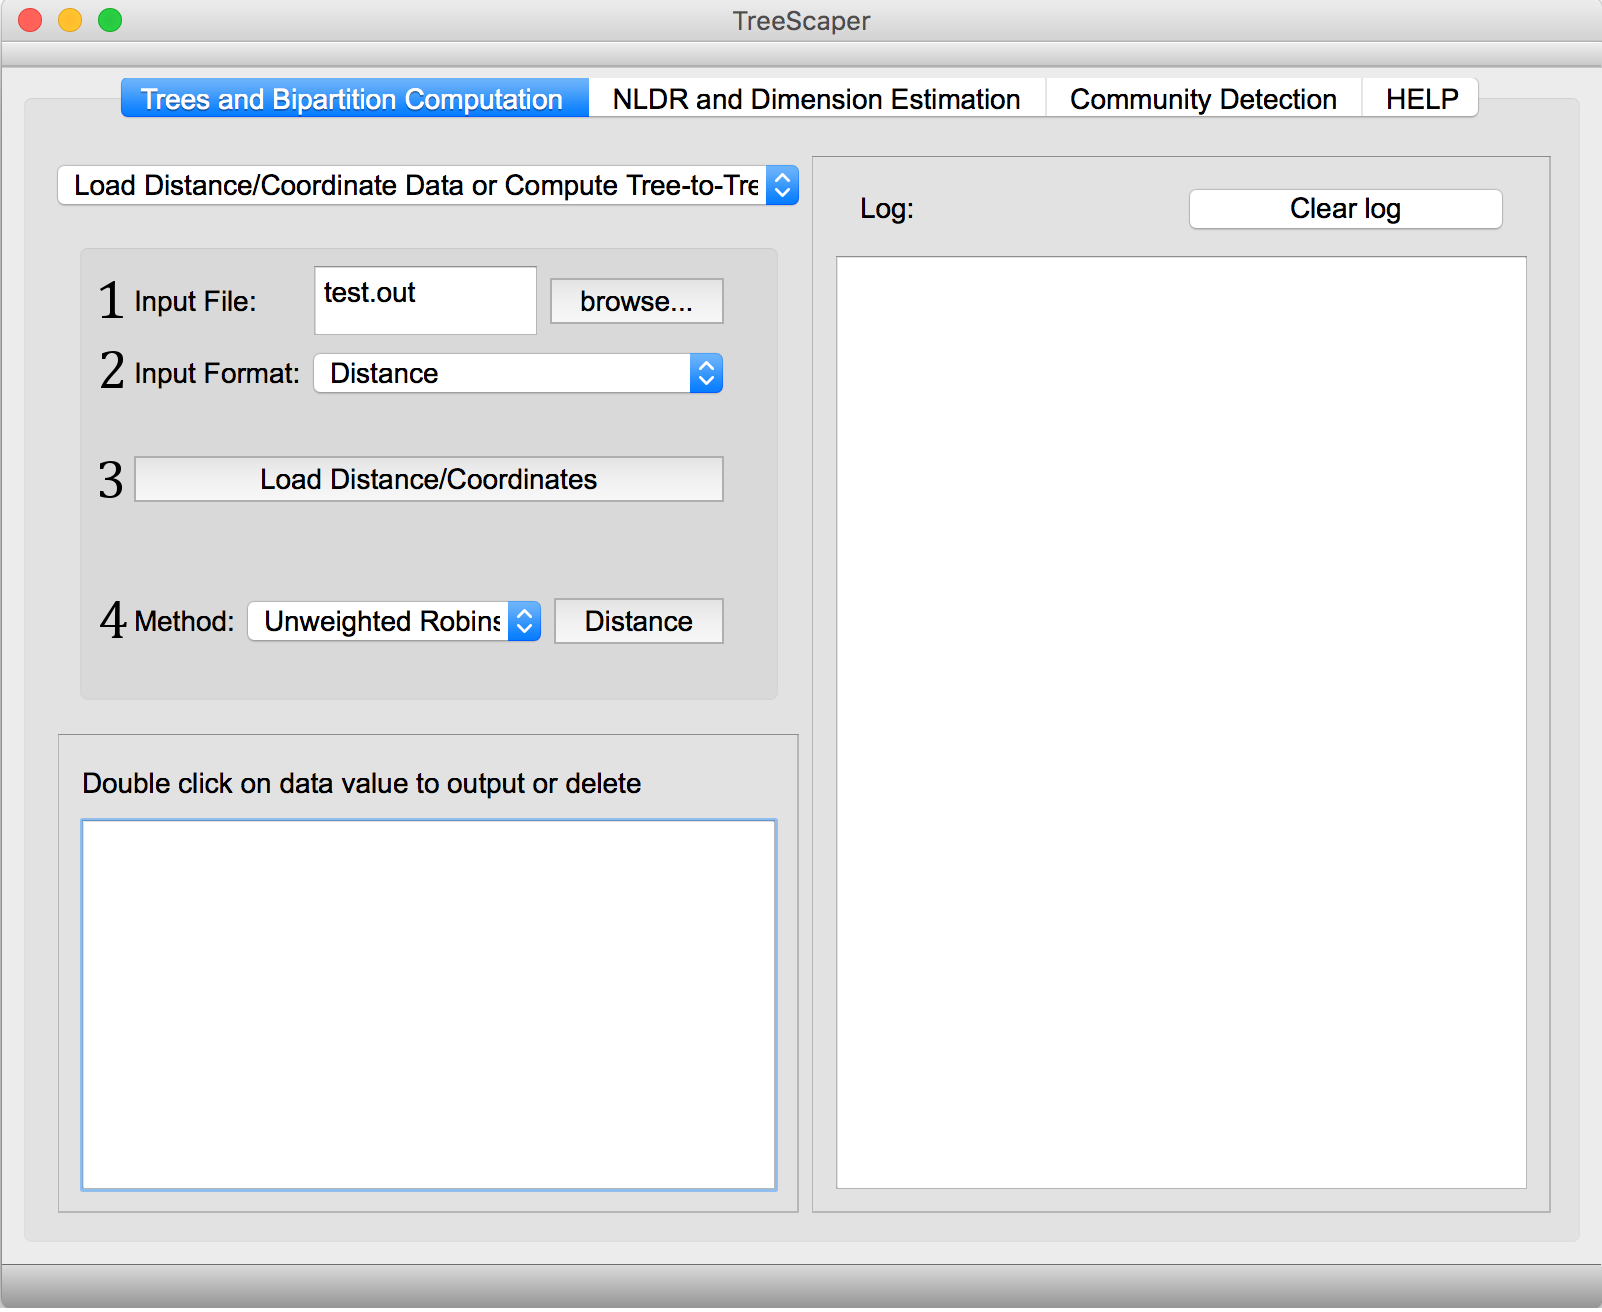
\includegraphics[scale=0.4]{imagesForManual/Figure10_6_1_5.png}
%\caption{}\label{fig10}
\end{figure}

The options in this pane allow tree-to-tree distances to either be computed from scratch (see~\ref{DistMenu4} below) or to be loaded from file if already computed (see~\ref{DistMenu1} -~\ref{DistMenu3} below). If loaded from file, any
distances may be used. If computed in TreeScaper, see the ``Method" dropdown for a list of
available distances. \\

\begin{enumerate}[{\bf 1-}]
\item {\bf [Input File]} -- Select the location of a file containing a distance matrix. The matrix needs to
be similar to the format of ``1000bp1L\_Unweighted RF-distance.out" -- a lower triangle tree-to-tree distance matrix. Negative values are not allowed. \label{DistMenu1}

\item {\bf [Input Format]} -- Select whether the input file is formatted for distances (the vast majority
of cases) or 2D/3D coordinates (when pre-computed). \label{DistMenu2}

\item {\bf [Load Distance/Coordinates]} -- Load the distance matrix or coordinates specified in the
``Input File" into memory. \label{DistMenu3}

\item {\bf [Method]} -- If computing tree-to-tree distances from scratch, choose a distance. Options
include Unweighted Robinson-Foulds, Weighted Robinson-Foulds, Matching, and SubtreePrune-Regraft (SPR) distances. As far as we know, TreeScaper is currently the only program
available that can calculate all of these distances. Click ``Distance" to compute the distance
matrix. \label{DistMenu4}
\end{enumerate}

%%%%%%%%%%%%%%%%%%%%%%%%%%%%%%%%%%%%%%%%%%%%%%%%%%%
% Convert Tree-to-Tree Distances to Affinities
\newpage
\subsubsection{Convert Tree-to-Tree Distances to Affinities}\label{subsubsect:ConvertDistToAffinity}

\begin{figure}[thbp!]\centering
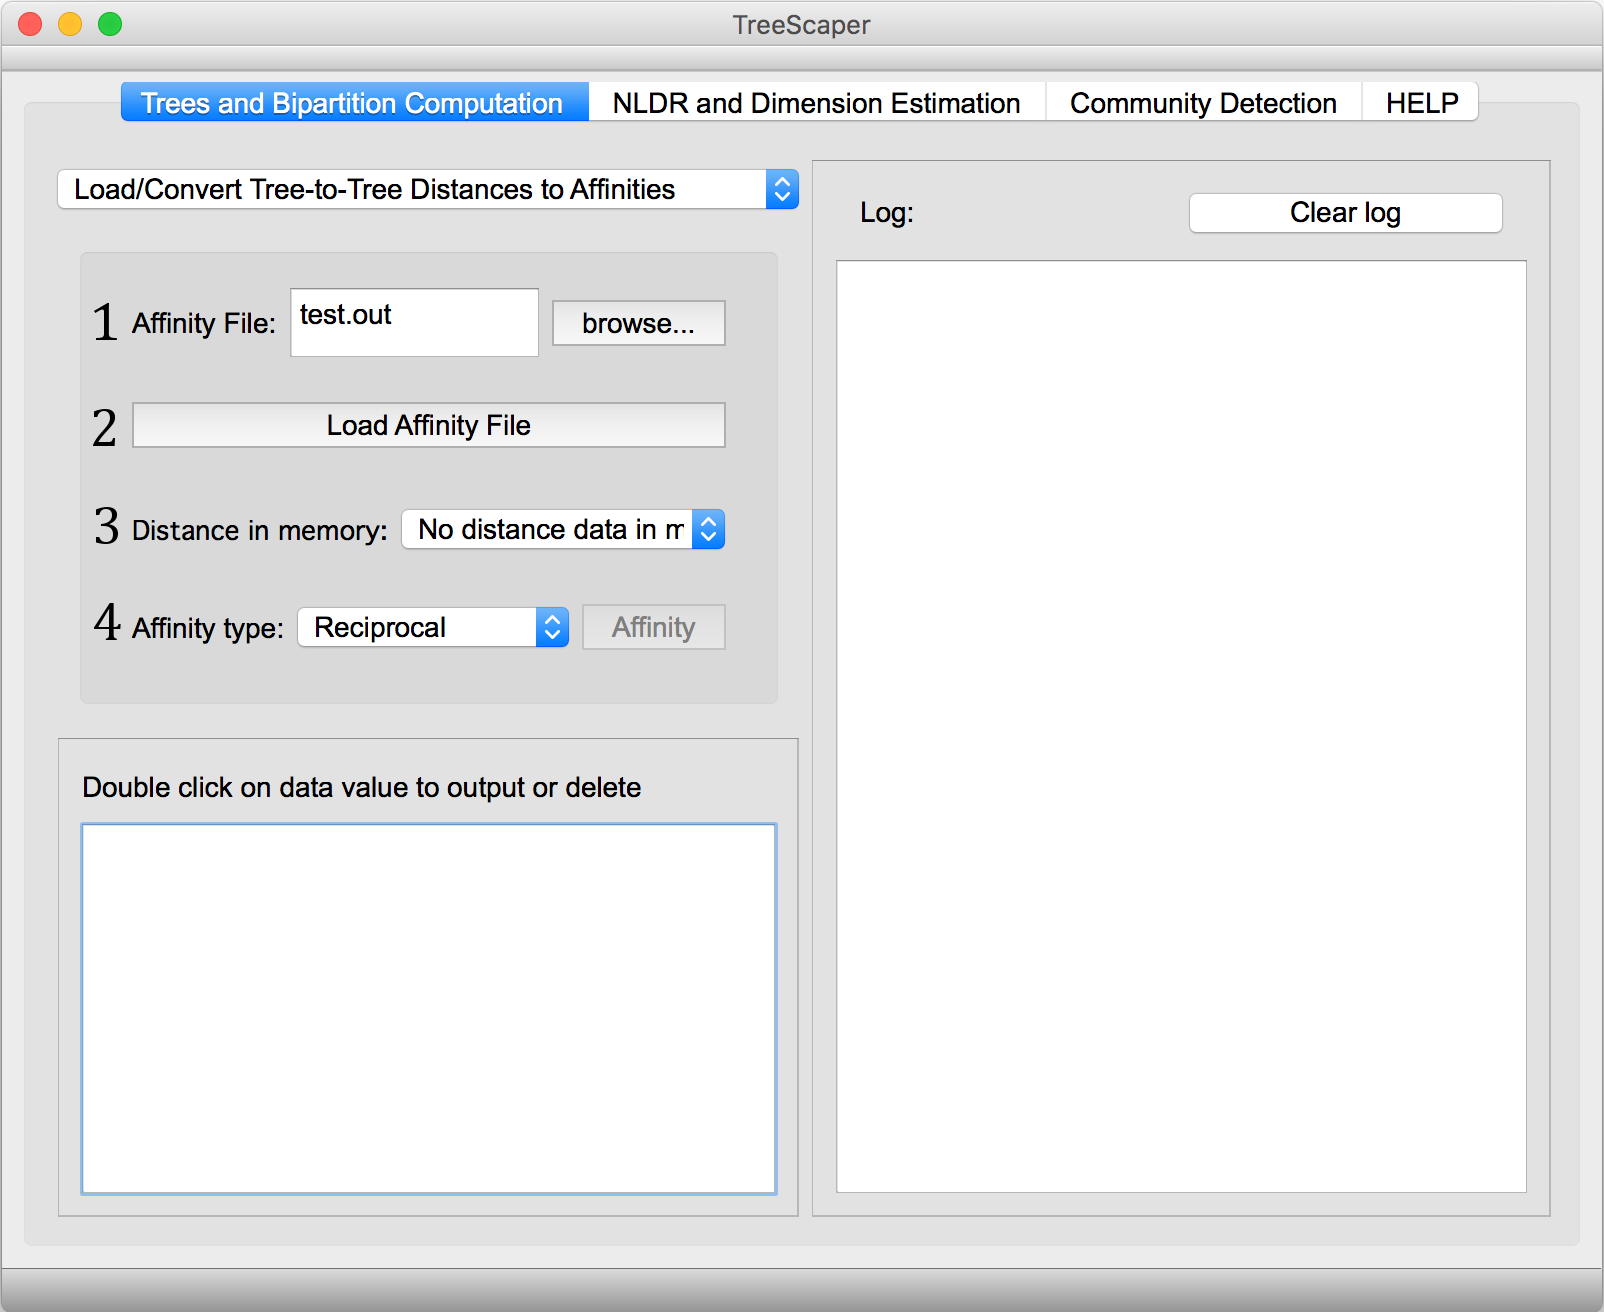
\includegraphics[scale=0.4]{imagesForManual/Figure11_6_1_6.png}
%\caption{}\label{fig11}
\end{figure}

In the topological networks used by TreeScaper, nodes correspond to sampled trees and edge
weights correspond to the affinity (or similarity) between pairs of sampled trees. Before
community detection can be performed on these networks, tree-to-tree distances must be
converted to affinities. TreeScaper allows users both to load pre-computed affinities from a
file (options~\ref{AffMenu1} and~\ref{AffMenu2} below) or to calculate affinities directly from distances in memory (options~\ref{AffMenu3} and~\ref{AffMenu4} below). \\

\begin{enumerate}[{\bf 1-}]
\item {\bf [Affinity File]} -- Although affinities may be calculated from a distance matrix stored in
memory, it�s also possible that you�ve previously calculated affinities and output that
information to a file. In such cases, you may select that file here using browse. \label{AffMenu1}

\item {\bf [Load Affinity File]} -- Load the chosen ``Affinity File" into memory. \label{AffMenu2}

\item {\bf [Distance in memory]} -- Select which distance matrix to use. If there is no distance matrix
in memory, the drop down box will read ``No distance data". \label{AffMenu3}

\item {\bf [Affinity type]} -- Choose how to transform the distance matrix to an affinity matrix.
``Reciprocal" computes the reciprocal of distance. ``Exponential" computes an exponential
transformation of the distance. \label{AffMenu4}
\end{enumerate}

%%%%%%%%%%%%%%%%%%%%%%%%%%%%%%%%%%%%%%%%%%%%%%%%%%%
% Dimension Estimation and NLDR
\newpage
\subsection{Nonlinear Dimensionality Reduction and Dimension Estimation}\label{subsect:DimEstNLDR}


%%%%%%%%%%%%%%%%%%%%%%%%%%%%%%%%%%%%%%%%%%%%%%%%%%%
% Nonlinear Dimensionality Reduction (NLDR)
\subsubsection{Nonlinear Dimensionality Reduction (NLDR)}\label{subsubsect:NLDR}

\begin{figure}[thbp!]\centering
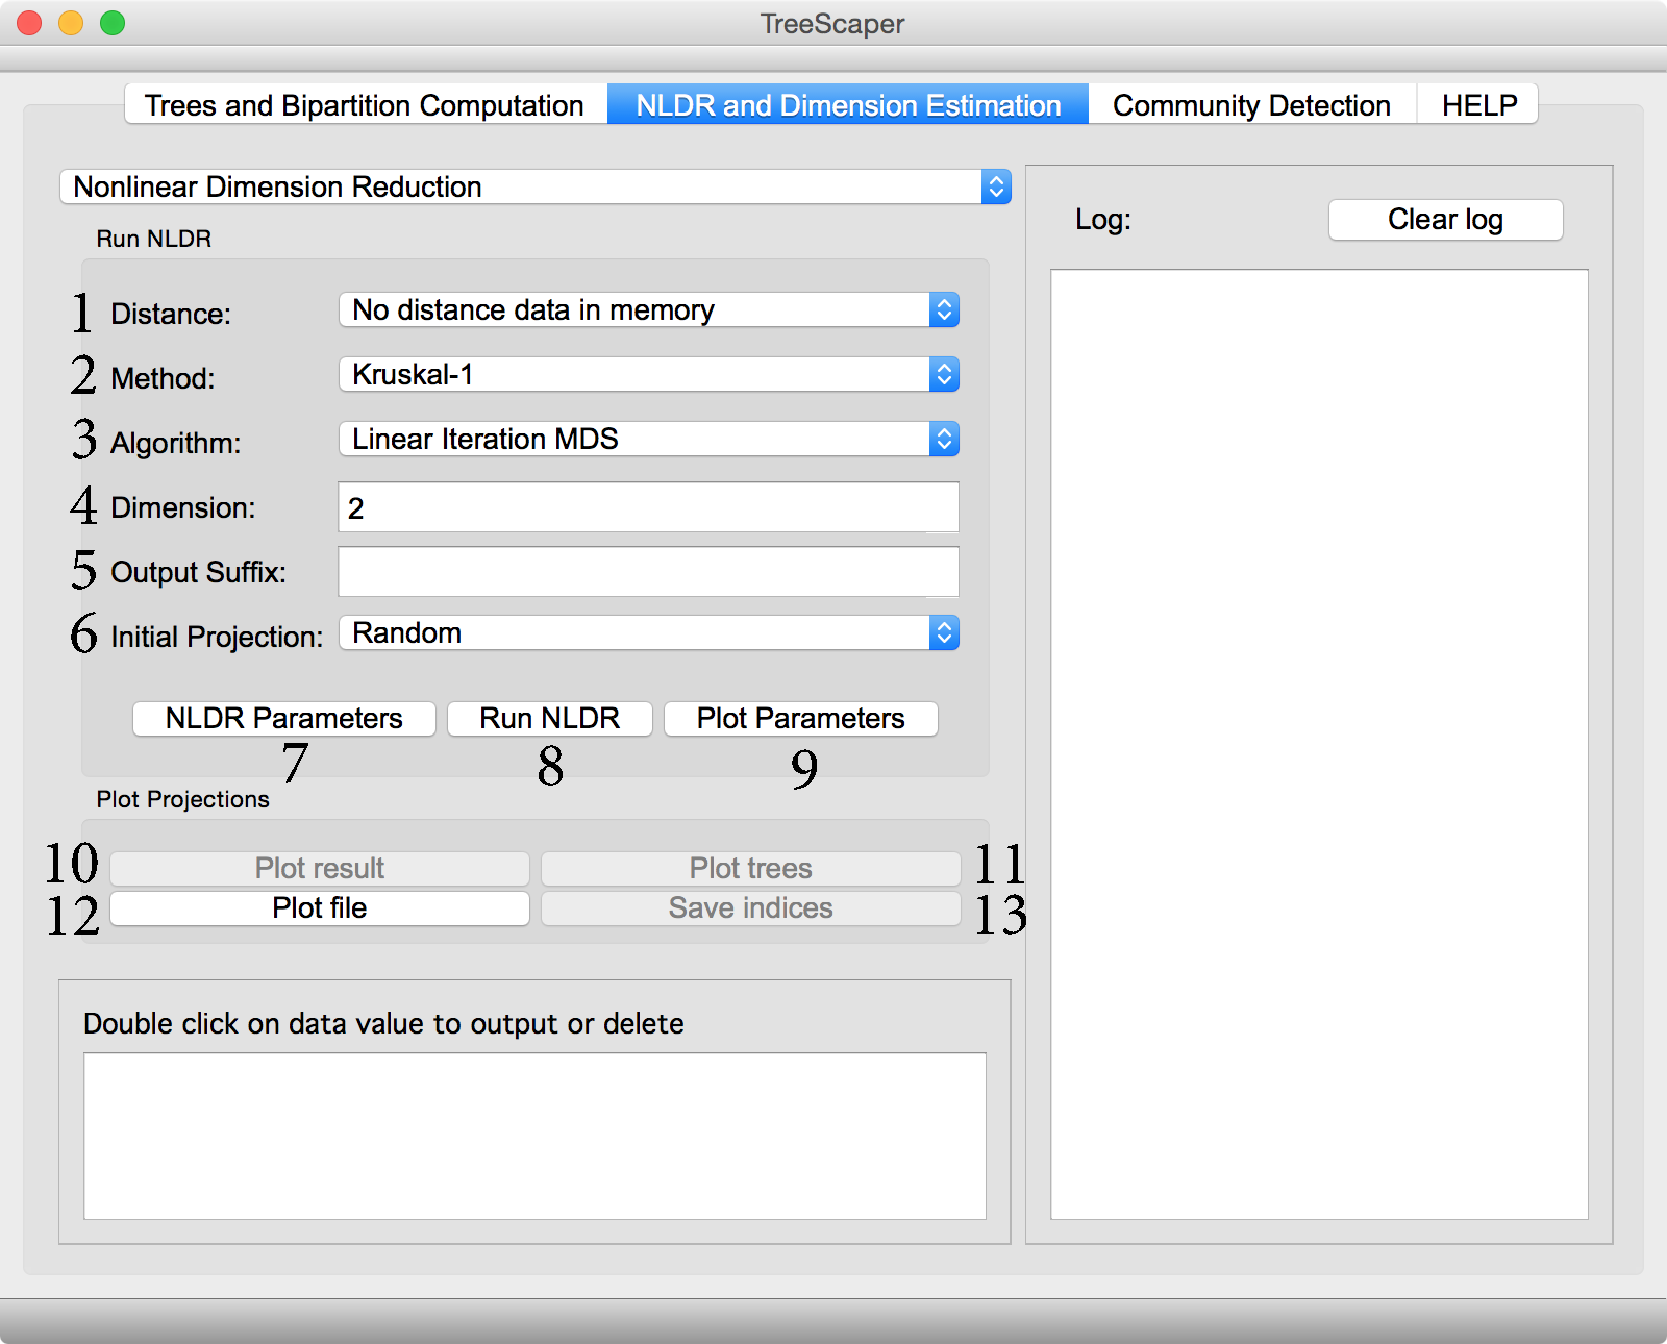
\includegraphics[scale=0.4]{imagesForManual/Figure12_6_2_1.pdf}
%\caption{}\label{fig12}
\end{figure}

NLDR seeks to find a low-dimensional representation that accurately reflects a set of highdimensional distances. TreeScaper allows users to run NLDR for any specified number of
dimensions, although points can only be visualized in $1-3$ dimensions. If more than $3$
dimensions are used when NLDR is run, only the first $3$ axes will be used in the plot. \\


\noindent{\it Run NLDR Panel}\\


\begin{enumerate}[{\bf 1-}]
\item {\bf [Distance]} -- Select a distance matrix from memory. See options in the ``Trees and
Bipartition Computation" tab to compute a distance matrix if one is not currently available in
memory.

\item {\bf [Method]} -- Select the method used for NLDR. Classic Scaling uses singular value
decomposition (SVD). Kruskal$-1$ uses Kruskal stress$-1$ as the stress function. Normalized
uses normalized stress. NLM uses Sammon nonlinear mapping. CCA uses curvilinear
component analysis.

\item {\bf [Algorithm]} -- Select the optimization algorithm. For Classic Scaling, the algorithm used is
always ``SVD". For Kruskal$-1$, the ``Stochastic" algorithm is not recommended because it is
slow. For Normalized, NLM and CCA, the �Linear Iteration MDS� algorithm is not available.
Linear iteration is used in the Hillis et al. paper~\ref{HHJA:2005}. ``Stochastic" uses a stochastic gradient descent algorithm and appears to have the best performance.

\item {\bf [Dimension]} -- Select the number of dimensions for the low-dimensional projection. Any
number of dimensions may be used, but only $1-3$ dimensions can be visualized.

\item {\bf [Output Suffix]} -- Choose a suffix to distinguish the output files when they have the same
name.

\item {\bf [Initial Projection]} --  This is the initial matrix used for the iteration. ``Random" means a
uniform random number is used. "Classic scaling" means the initial matrix is the result of
classic scaling:\\

\begin{sloppypar}\noindent{\color{blue}\url{https://en.wikipedia.org/wiki/Multidimensional_scaling#Classical_multidimensional_scaling}}\\ \end{sloppypar}

Usually, initialization with classic scaling makes the algorithm converge quickly.

\item {\bf [NLDR parameters]} -- Clicking this button opens a dialog box with a variety of specific
parameters that can be adjusted for each of the NLDR methods.

\item {\bf [Run NLDR]} -- Clicking this button uses the chosen NLDR method and optimization
algorithm to project trees into low-dimensional space. The projection can then be visualized
in TreeScaper directly (see below) or TreeScaper can output coordinate files, so that you can
use third party plotting packages like Matlibplot to create publication quality figures in a
number of output formats (See output files section).

\item {\bf [Plot parameters]} -- Click this and a dialog box will appear. Options in this box allow the
user to customize plots of NLDR projections. Click ``apply" to save any changes made to the
parameters. Here are details on some parameters of greatest practical interest: \\

A drop down box in the ``Plot" section that allows the user to select \ul{Points} or \ul{Convex\_Hull}.
\ul{Points} displays each tree as a separate point, while \ul{Convex\_Hull} displays each cluster of trees
as a convex hull. \\

In the ``Plot" section, the user can define a desired number of clusters in which to group the
trees. Each cluster will be given a unique color. Click {\bf OK} to save the number of clusters. \\

The user can set the range of tree indices in each cluster manually using the ``range" column
under ``Cluster index". These ranges can either be consecutive with only the beginnings and
endings specified (e.g., $1-10$) or they can consist of a comma-separated list of nonconsecutive indices (e.g., $1, 3, 6, 9, 14$). Alternatively, users can check ``step size" and simply
specify the number of trees to be in each cluster. The ``step size" option will start at $0$ and
increase by the step size to create the tree index range for each cluster. If the largest index is
greater than the number of trees in the tree set, this error will appear in the log: ``error: the
largest index should not be greater than the number of points!" If the largest index is less than
the number of trees in the tree set, the trees whose indices were excluded will not be plotted
in the NLDR projection. If the parameters are changed such that indices are missing between
$0$ and the largest index, TreeScaper will most likely crash. {\it Make sure that all tree indices are
assigned to a cluster.} \\
\end{enumerate}


\noindent{\it Plot Projections Panel}\\


\begin{enumerate}[{\bf 1-}]
\setcounter{enumi}{9}
\item {\bf [Plot Result]} -- Creates a $1-$, $2-$, or $3-$dimensional representation of the NLDR projection. To the left of the figure is a legend showing the colors assigned to the clusters. On a Mac,
clicking and dragging allows the plot to be rotated in $3$ dimensions. Holding down the
Control key while clicking and dragging rotates the plot in $2$ dimensions. Holding down the
Shift key while clicking and dragging repositions the plot. Pressing the Shift and R keys
together will toggle in between two functions for clicking and dragging: (1) rotating the plot
or (2) selecting points in the plot. \label{NLDRmenu10}

\item {\bf [Plot trees]} --  {\it Note: this function only works for the Mac version currently.} If points in the
plot have been selected (see~\ref{NLDRmenu10} above), clicking this button will separately display each selected tree. For each displayed tree, scrolling up and down will zoom in and out. Holding
down either the Option or Command keys while clicking and dragging will reposition the
tree. If some labels are not initially visible, try zooming in.

\item {\bf [Plot File]} -- Select a file containing a previously computed NLDR projection and plot it.
These files contain the coordinates in low-dimensional space and have \_COR\_ in their
names.

\item {\bf [Save Indices]} -- If points in the plot have been selected (see~\ref{NLDRmenu10} above), clicking this button will output the selected trees to a file. \\
\end{enumerate}


\noindent{\it Output Files}\\


\noindent Each time an NLDR analysis is run in TreeScaper, a series of output files are automatically
created. These files have names indicating the name of the tree set, the tree-to-tree distance,
the NLDR method, and the optimization algorithm. If NLDR is run multiple times and any of
these parameters are changed, a new set of files will be created. If NLDR is run multiple times
with the same parameters, only the final run will be saved. \\


\noindent {\bf $^{*}$\_$^{*}$D\_$^{*}$\_COR\_$^{*}$.out:} The $*$s represent the filename, dimension, method and algorithm. This file contains the NLDR coordinates. Each row represents a sampled tree and is depicted as a
point in low-dimensional space. {\it For more customized NLDR plots, users can simply read these
coordinates into software packages with greater plotting flexibility (e.g., R) and adjust options
as they see fit.} \\


\noindent {\bf $^{*}$\_$^{*}$D\_$^{*}$\_DIS\_$^{*}$.out:} The Euclidean distance matrix of the NLDR coordinates. \\


\noindent {\bf $^{*}$\_$^{*}$D\_$^{*}$\_STR\_$^{*}$.out:}  The value of stress function after optimization. \\


\noindent {\bf $^{*}$\_$^{*}$D\_$^{*}$\_TIM\_$^{*}$.out:} The time cost. \\


\noindent {\bf $^{*}$\_$^{*}$D\_$^{*}$\_1NN\_$^{*}$.out:} The first element is the 1nn percentage of the original distance matrix. The second element is the 1nn percentage of the result distance matrix. \\


\noindent {\bf $^{*}$\_$^{*}$D\_$^{*}$\_CON\_$^{*}$.out:} The continuity. The first column is the number of neighbors considered. The second column is the continuities. \\


\noindent {\bf $^{*}$\_$^{*}$D\_$^{*}$\_TRU\_$^{*}$.out:} The trustworthiness. The first column is the number of neighbors considered. The second column is the trustworthiness. \\


%%%%%%%%%%%%%%%%%%%%%%%%%%%%%%%%%%%%%%%%%%%%%%%%%%%
% Dimension Estimation
\newpage
\subsubsection{Dimension Estimation}\label{subsubsect:DimEst}

\begin{figure}[thbp!]\centering
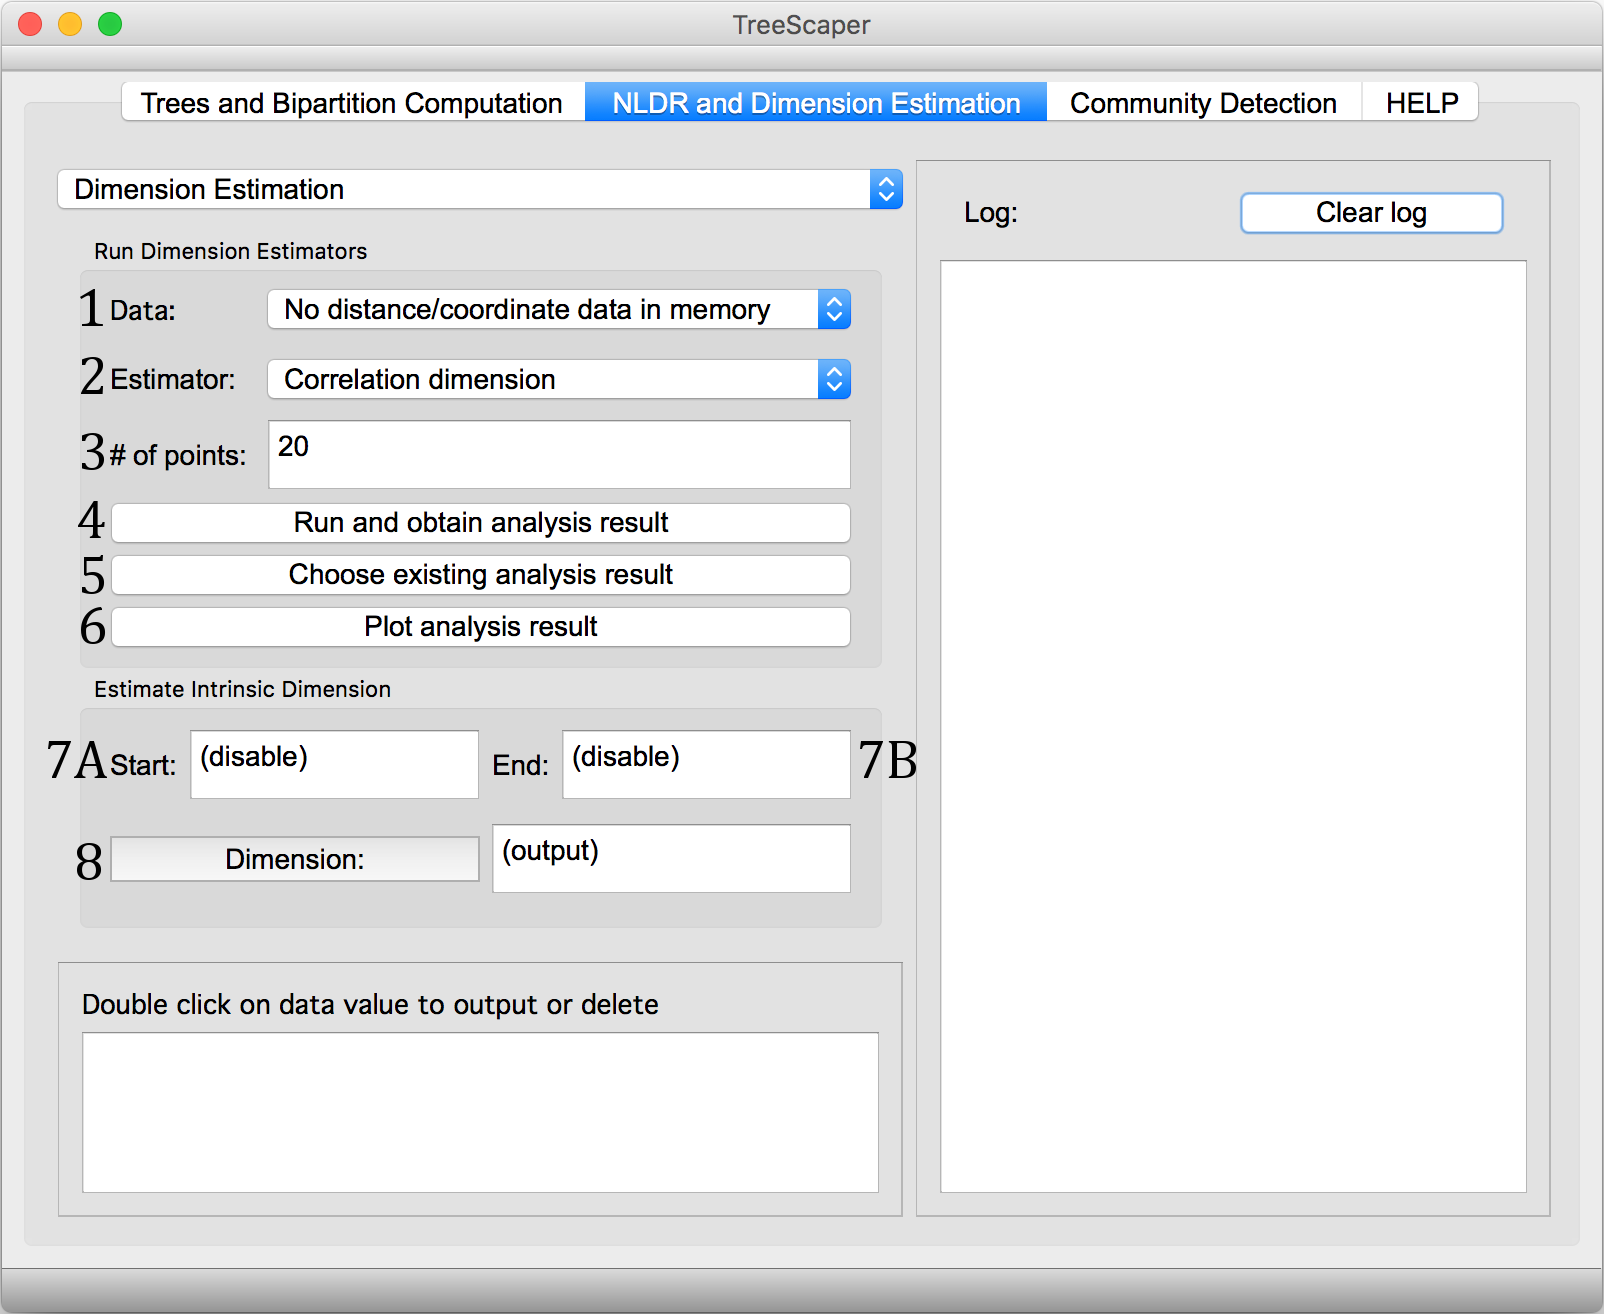
\includegraphics[scale=0.4]{imagesForManual/image_8.png}
%\caption{}\label{fig13}
\end{figure}

In addition to conducting NLDR analyses, TreeScaper allows users to estimate the intrinsic
dimensionality of their data. By doing so, one can gain a sense for how much information is
lost when projecting into lower dimensional space. \\


\noindent{\it Run Dimension Estimators}\\


\begin{enumerate}[{\bf 1-}]
\item {\bf [Data]} -- Select a set of tree-to-tree distances from this dropdown menu.

\item {\bf [Estimator]} -- Select one of three dimension estimators: correlation dimension, maximum
likelihood, or nearest neighbor estimator.

\item {\bf [\# of points]} -- For the maximum likelihood and nearest neighbor estimators, this value
determines the number of neighbors considered. For correlation dimension, this value
represents the number of points used in the interval.

\item {\bf [Run and obtain analysis results]} -- Run the dimension estimator.

\item {\bf [Choose existing analysis result]} -- Choose a previous dimension estimation output file for
analysis.

\item {\bf [Plot analysis result]} -- Plot a figure of the output file. \\
\end{enumerate}


\noindent{\it Estimate Intrinsic Dimension} \\


\begin{enumerate}[{\bf 7}]
\item {\bf A- [Start] and B- [End]} -- Choose the range of the interval used to compute dimension.
\end{enumerate}


\begin{enumerate}[{\bf 8-}]
\item {\bf [Dimension]} -- Estimate the dimension in the given interval. For the nearest neighbor and
correlation dimension estimators, the dimension is the slope. For the maximum likelihood
estimator, the dimension is the mean. \\
\end{enumerate}


\noindent{\it Output files} \\


\noindent {\bf $^{*}$\_CORR\_DIM\_logvslog.out:} Correlation dimension output. The $^{*}$ represents the filename. If one plots a figure of the first column versus the second column, the slope of the curve is the correlation dimension. \\


\begin{sloppypar}\noindent {\bf $^{*}$\_CORR\_DIM\_deri\_logvslog.out:} Correlation dimension output. This is the slope of ``$^{*}$\_CORR\_DIM\_logvslog.out" and is given by using the central difference method. \\ \end{sloppypar}


\noindent {\bf $^{*}$\_MLE\_DIM\_k.out:} Maximum likelihood estimator output. The $i^{th}$ row represents the dimension given by considering the $k$ nearest neighbor. The dimension is the mean of some interval of the neighborhood. \\


\begin{sloppypar}\noindent {\bf $^{*}$\_MLE\_DIM\_dim.out:} Maximum likelihood estimator output. It is the mean of the $^{*}$\_MLE\_DIM\_k.out. \\ \end{sloppypar}


\noindent {\bf $^{*}$\_NN\_DIM\_logvslog.out:} Nearest neighbor estimator output. If one plots a figure of the first column versus the second column, the slope of the curve is the nearest neighbor dimension. \\

\begin{sloppypar}\noindent {\bf $^{*}$\_NN\_DIM\_deri\_logvslog.out:} Nearest neighbor estimator output. This is the slope of ``$^{*}$\_NN\_DIM\_logvslog.out� and is given by using the central difference method. \\ \end{sloppypar}

%%%%%%%%%%%%%%%%%%%%%%%%%%%%%%%%%%%%%%%%%%%%%%%%%%%
% Community Detection
\newpage
\subsection{Community Detection}\label{subsect:CommunityDetectionMenu}


%%%%%%%%%%%%%%%%%%%%%%%%%%%%%%%%%%%%%%%%%%%%%%%%%%%
% Community Detection on a Bipartition-Covariance Network
\subsubsection{Community Detection in Bipartition-Covariance Networks}\label{subsubsect:CommunityDetectionBipartCovMenu}


\begin{figure}[thbp!]\centering
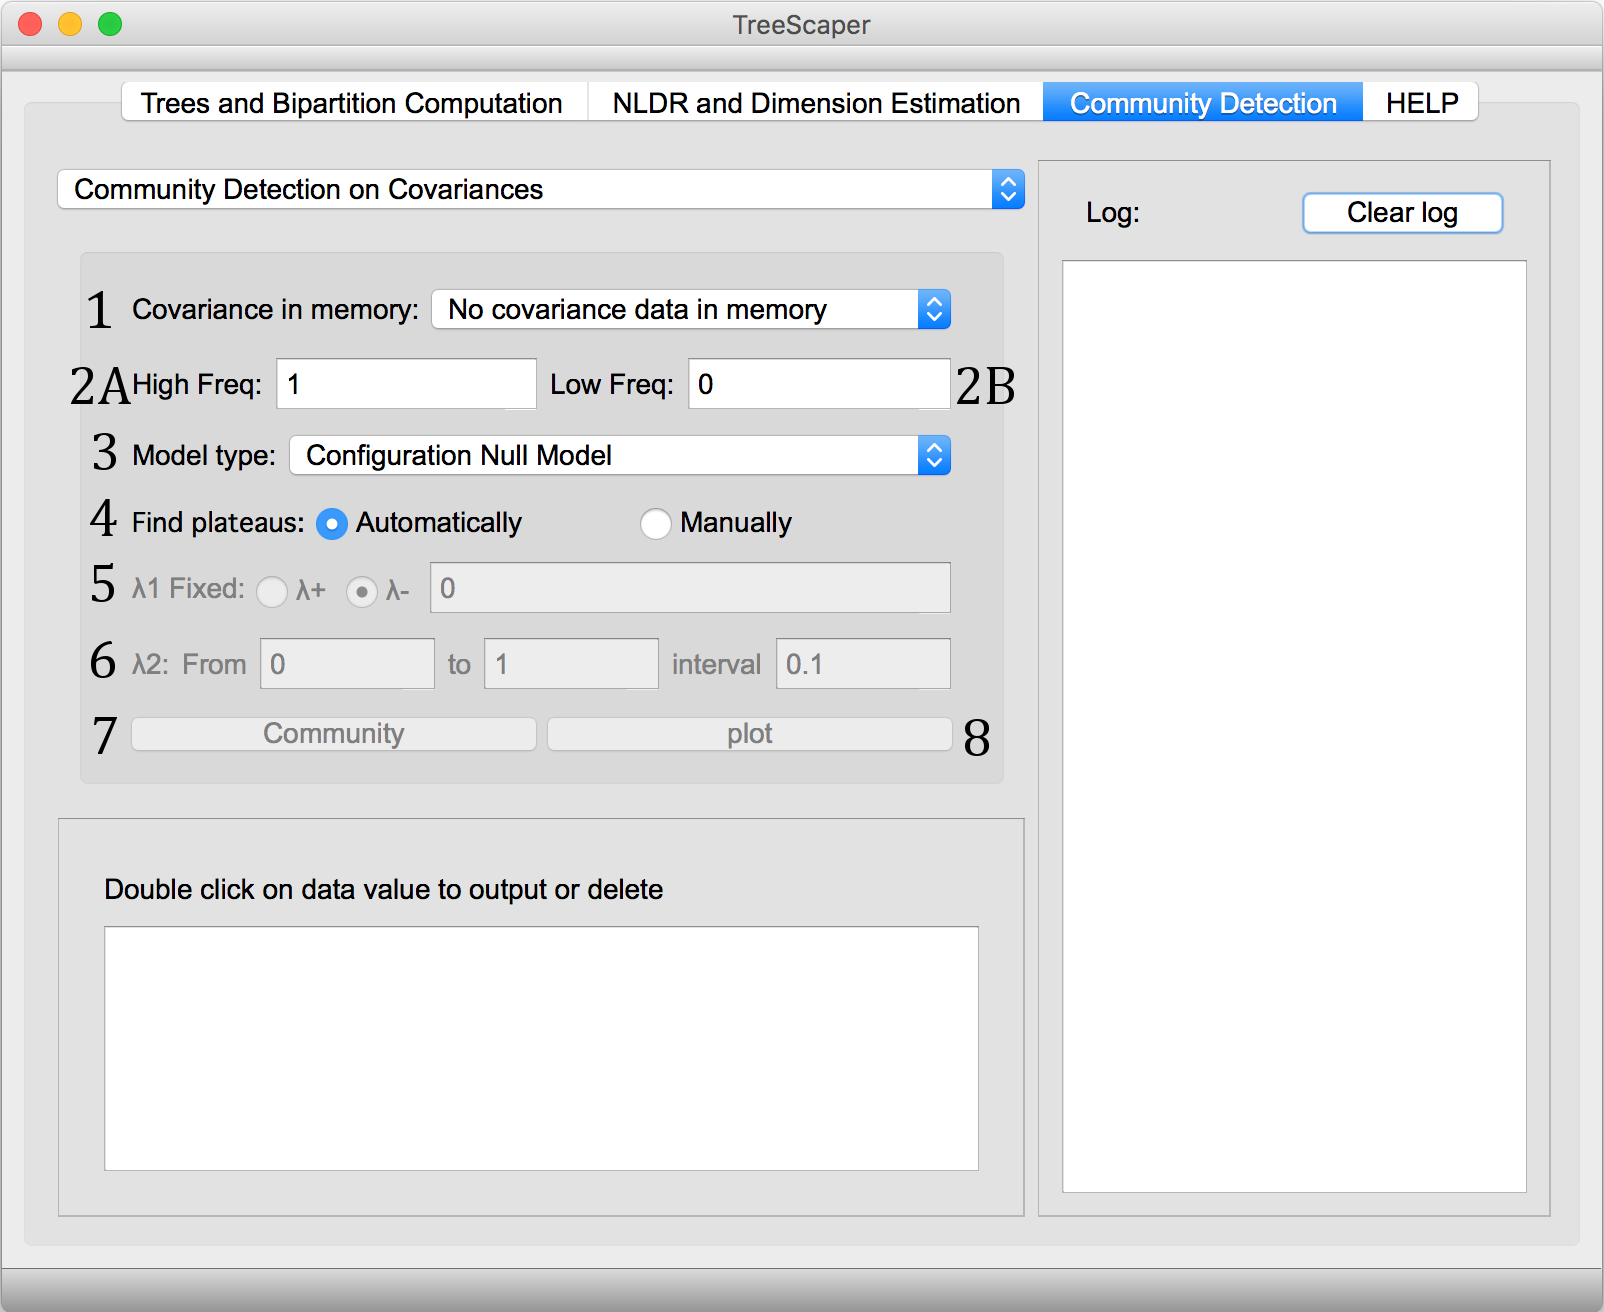
\includegraphics[scale=0.4]{imagesForManual/image_9.png}
%\caption{}\label{fig14}
\end{figure}

In the bipartition covariance network, nodes correspond to bipartitions and the weights of
edges connecting these nodes correspond to their covariance in presence/absence across tree
samples (Fig.~\ref{fig3}). Community detection in these covariance networks attempts to group
bipartitions that have positive covariances and separate bipartitions that have negative
covariances. \\

\begin{enumerate}[{\bf 1-}]
\item {\bf [Covariance in memory]} -- Select the covariance matrix in memory to use for community
detection. If there is no covariance matrix in memory, the drop down box will read ``No
covariance data".

\item {\bf A- [High Freq] and B- [Low Freq]} -- High and low frequency bipartitions often have small
covariances with every other bipartition in the tree set, making them very difficult to assign to
a particular community. Because these bipartitions do not represent strongly supported
conflicting signal, the user may want to filter these bipartitions out of the analysis. ``High
Freq" specifies the frequency above which bipartitions are filtered out. ``Low Freq" specifies
the frequency below which bipartitions are filtered out.

\item {\bf [Model type]} -- Select the model to use for community detection. Options are the
Configuration Null Model, the Constant Potts Model, the Erd\'{o}s-R\'{e}nyi  Model, and the No
Null Model. Each of these models is described in more detail in Appendix~\ref{appendix:CDModels}.

\item {\bf [Find Plateaus]} -- Several community detection models depend on tuning parameters to
determine the scale at which communities are detected. In order to determine which values
of these parameters are most appropriate, we can look for parameter ranges where
community structure remains stable. When plotting community number against parameter
values, the largest of these plateaus of intrinsic stability is preferred. If ``Automatically" is
selected, TreeScaper tries to find the intrinsic community structure of the network by
efficiently testing different values of the tuning parameters. In this automated setting,
TreeScaper looks for the largest plateau across values of tuning parameters that produce nontrivial community structures. Community structures are trivial if all bipartitions are placed in
a single community or if every bipartition is placed in its own community. If ``Manually" is
selected, the user searches for the intrinsic community structure by specifying which
parameter values are to be tested. \\
\end{enumerate}


\noindent If ``Manually" is selected in the ``Find Plateaus" section: \\


\begin{enumerate}[{\indent\bf 1-}]
\setcounter{enumi}{4}

\item {\bf [$\mathbf{\lambda1}$ fixed]} -- If the Constant Potts Model (CPM) is used, or the Configuration Null
Model (CNM) or Erdos-R�nyi Null Model (ERNM) are used and the trees are fully
binary, only the difference between $\lambda^{+}$ and $\lambda^{-}$ matters for community detection.
Therefore, if one wishes to vary the $\lambda$ values to see how they affect community
detection, one can fix one of the $\lambda$ values and vary the other. This option allows the
user to select whether to fix $\lambda^{+}$ or $\lambda^{-}$.

\item {\bf [$\mathbf{\lambda2}$]} -- For the $\lambda$ parameter that will be varied, the user can choose the range of values to test and the interval separating consecutive values. To find the intrinsic
community structure of the network, vary the $\lambda$ parameter such that at one extreme,
each node is in its own community, and at the other extreme, all the nodes are
grouped into a single community. As with automatic community detection, the
intrinsic community structure can be chosen by looking for the largest range of $\lambda$
values that produces the same non-trivial community structure (i.e., the largest
plateau).
\end{enumerate}


\begin{enumerate}[{\bf 7-}]
\item {\bf [Community]} -- Runs community detection for a set of $\lambda$ values. \\
\end{enumerate}


If ``Automatically" is selected, the lambda values tested and the largest plateaus are
output to the log. For the plateaus, the ``Lower Bound" range is a conservative estimate for
the size of the plateau, while the ``Upper Bound" is each plateau�s largest possible size. If the
lower bound of the largest plateau is larger than the upper bound of the second largest
plateau, the user can be confident in the designation of a single plateau as the largest.
Automatic search does not work for non-binary trees when the CNM or ERNM models are
used. If ``Manually" is selected, the community structure detected for each $\lambda$ value (i.e., the
node indices placed in each community) is also output to the log. \\


\begin{sloppypar}Once community detection is complete, a summary of the community detection
results will be written to file. The name of the file is listed at the end of the log. The
summary will be a tab delimited file in the format of ``1000bp1L\_unrooted\_unweighted\_Covariance\_Matrix\_community\_auto\_results.out".  The first row contains numbers used to label each unique community structure. This number
starts at $0$ and increases by $1$ every time a unique community structure is found. The second
row contains each of the tested $\lambda2$ values. The third row contains the number of
communities. \\ \end{sloppypar}


\noindent\ul{\bf Note:} TreeScaper currently does not support use of the CNM or ERNM models for tree sets with non-binary trees. In these cases, the simple difference between $\lambda^{+}$ and $\lambda^{-}$ is not all that matters. Both $\lambda^{+}$ and $\lambda^{-}$ need to be varied independently to find a two-dimensional plateau. Given the complexity of this problem, we have not yet attempted an implementation. \\


\begin{enumerate}[{\bf 8-}]
\item {\bf [Plot]} -- Generate a plot of the community labels, number of communities, and the
modularities for different values of $\lambda$. These plots help the user to identify plateaus. \\
\end{enumerate}


%%%%%%%%%%%%%%%%%%%%%%%%%%%%%%%%%%%%%%%%%%%%%%%%%%%
% Community Detection on a Topological Network
\newpage
\subsubsection{Community Detection in Topological Affinity Networks}\label{subsubsect:CommunityDetectionTopologicalAffinityMenu}


\begin{figure}[thbp!]\centering
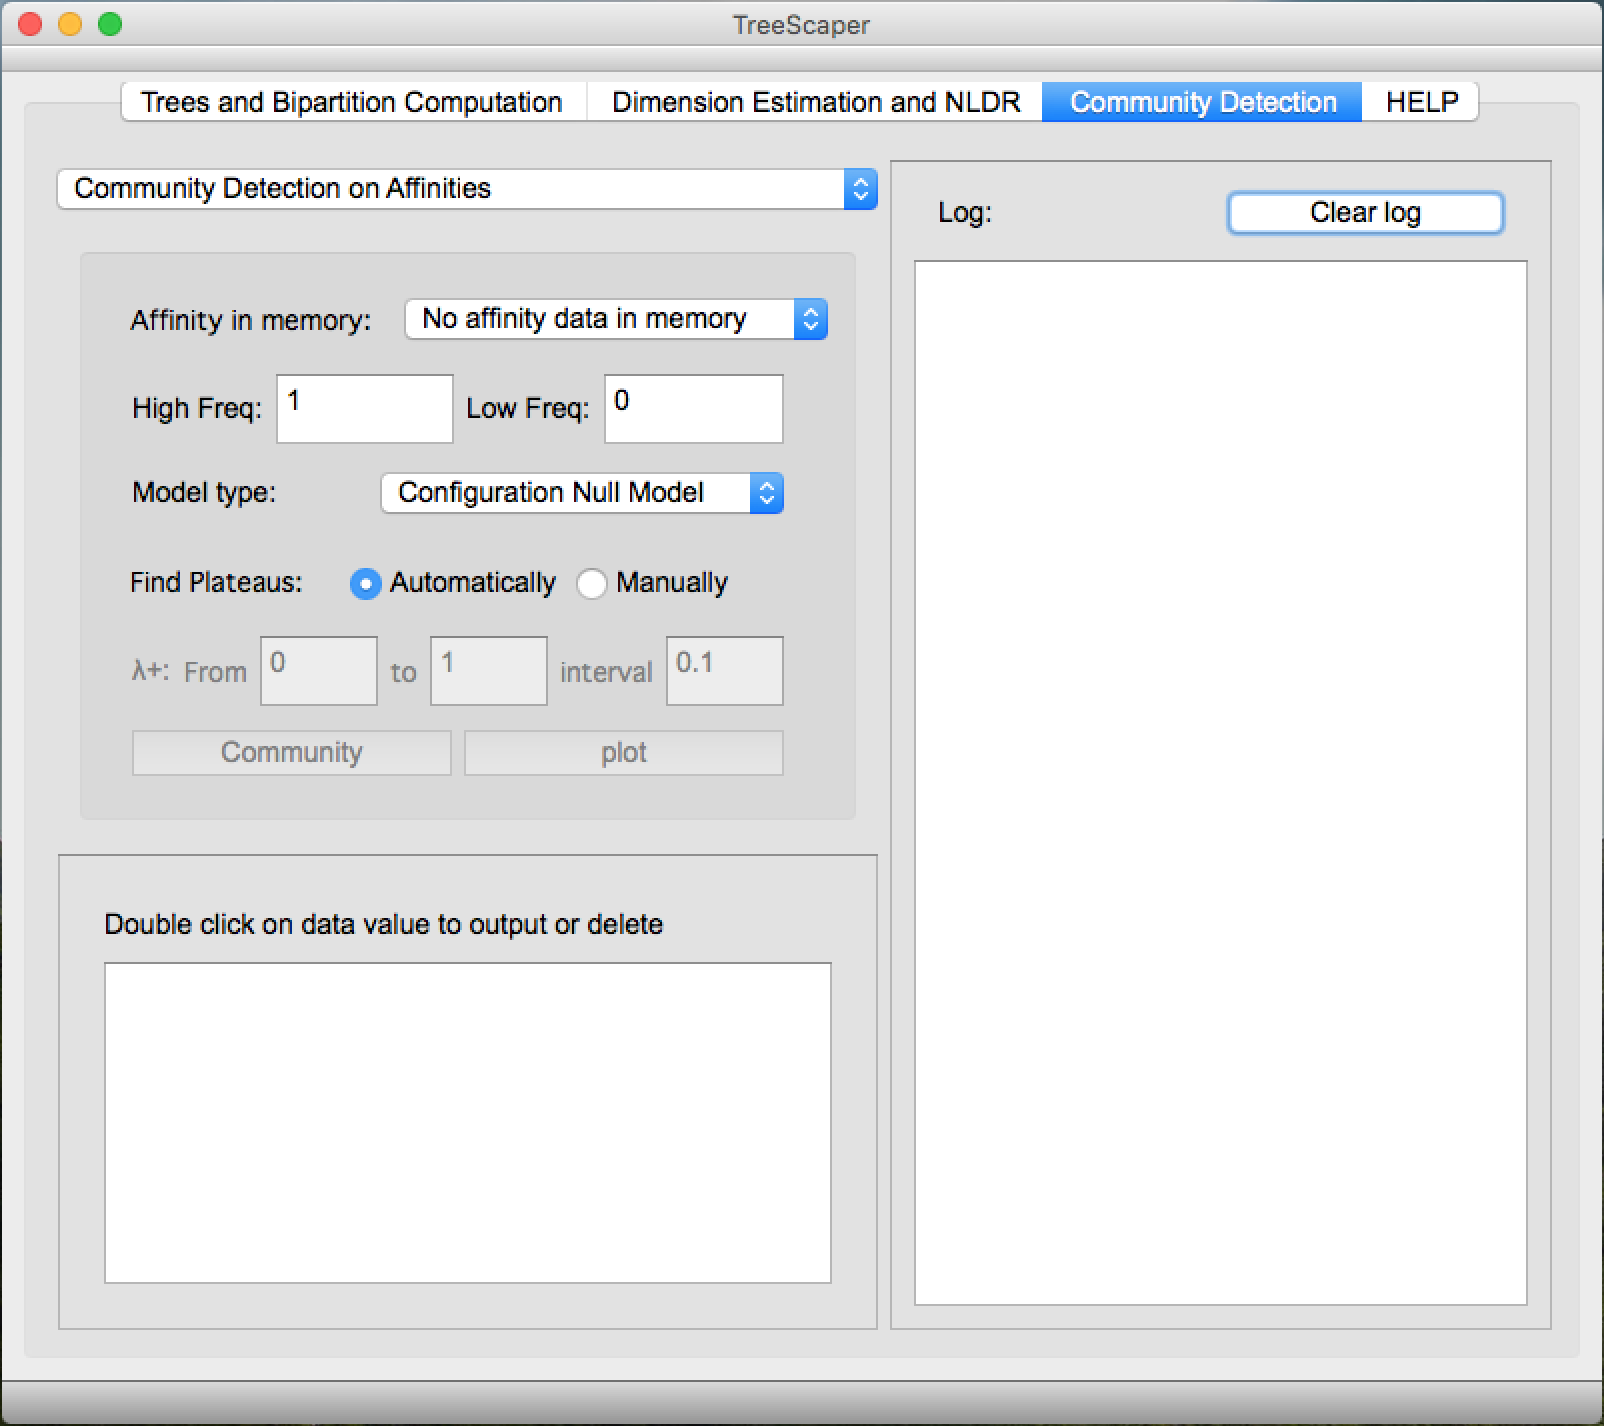
\includegraphics[scale=0.4]{imagesForManual/image_10.png}
%\caption{}\label{fig16}
\end{figure}


In topological networks, nodes represent individual topologies and edge weights correspond
to the similarity (or affinity) between each pair of topologies (Fig.~\ref{fig2}). Community detection
in these affinity networks attempts to find community boundaries that group similar
topologies and separate those that are dissimilar. \\


Most of the community detection menus for the affinity matrices are the same as those for
the covariance matrices. The community detection models are also the same, with two
exceptions. First, the $\lambda^{-}$ values are not applicable because there are no negative edges in the affinity matrices. Second, {\it the most interesting community structure for affinity matrices often
corresponds to the second largest plateau.} This plateau is of particular interest when there are
many trees in the tree set with identical topologies, and a discrete tree-to-tree distance (e.g.,
unweighted Robinson-Foulds, matching, or SPR) is used. In this situation, all duplicate tree
topologies will have a zero distance. If a wide range of parameter space is explored, the largest
plateau will often correspond to a community structure where every unique topology is
placed in its own community, which should generally be considered a trivial solution. This
community structure is not usually of much biological interest, because it is equivalent to a
simple list of the number of unique topologies and their frequencies with no information
about affinity. \\


%%%%%%%%%%%%%%%%%%%%%%%%%%%%%%%%%%%%%%%%%%%%%%%%%%%
% COMMAND-LINE TREESCAPER
%%%%%%%%%%%%%%%%%%%%%%%%%%%%%%%%%%%%%%%%%%%%%%%%%%%
\newpage
\section{COMMAND-LINE TREESCAPER}\label{sect:CLV}

\begin{figure}[thbp!]\centering
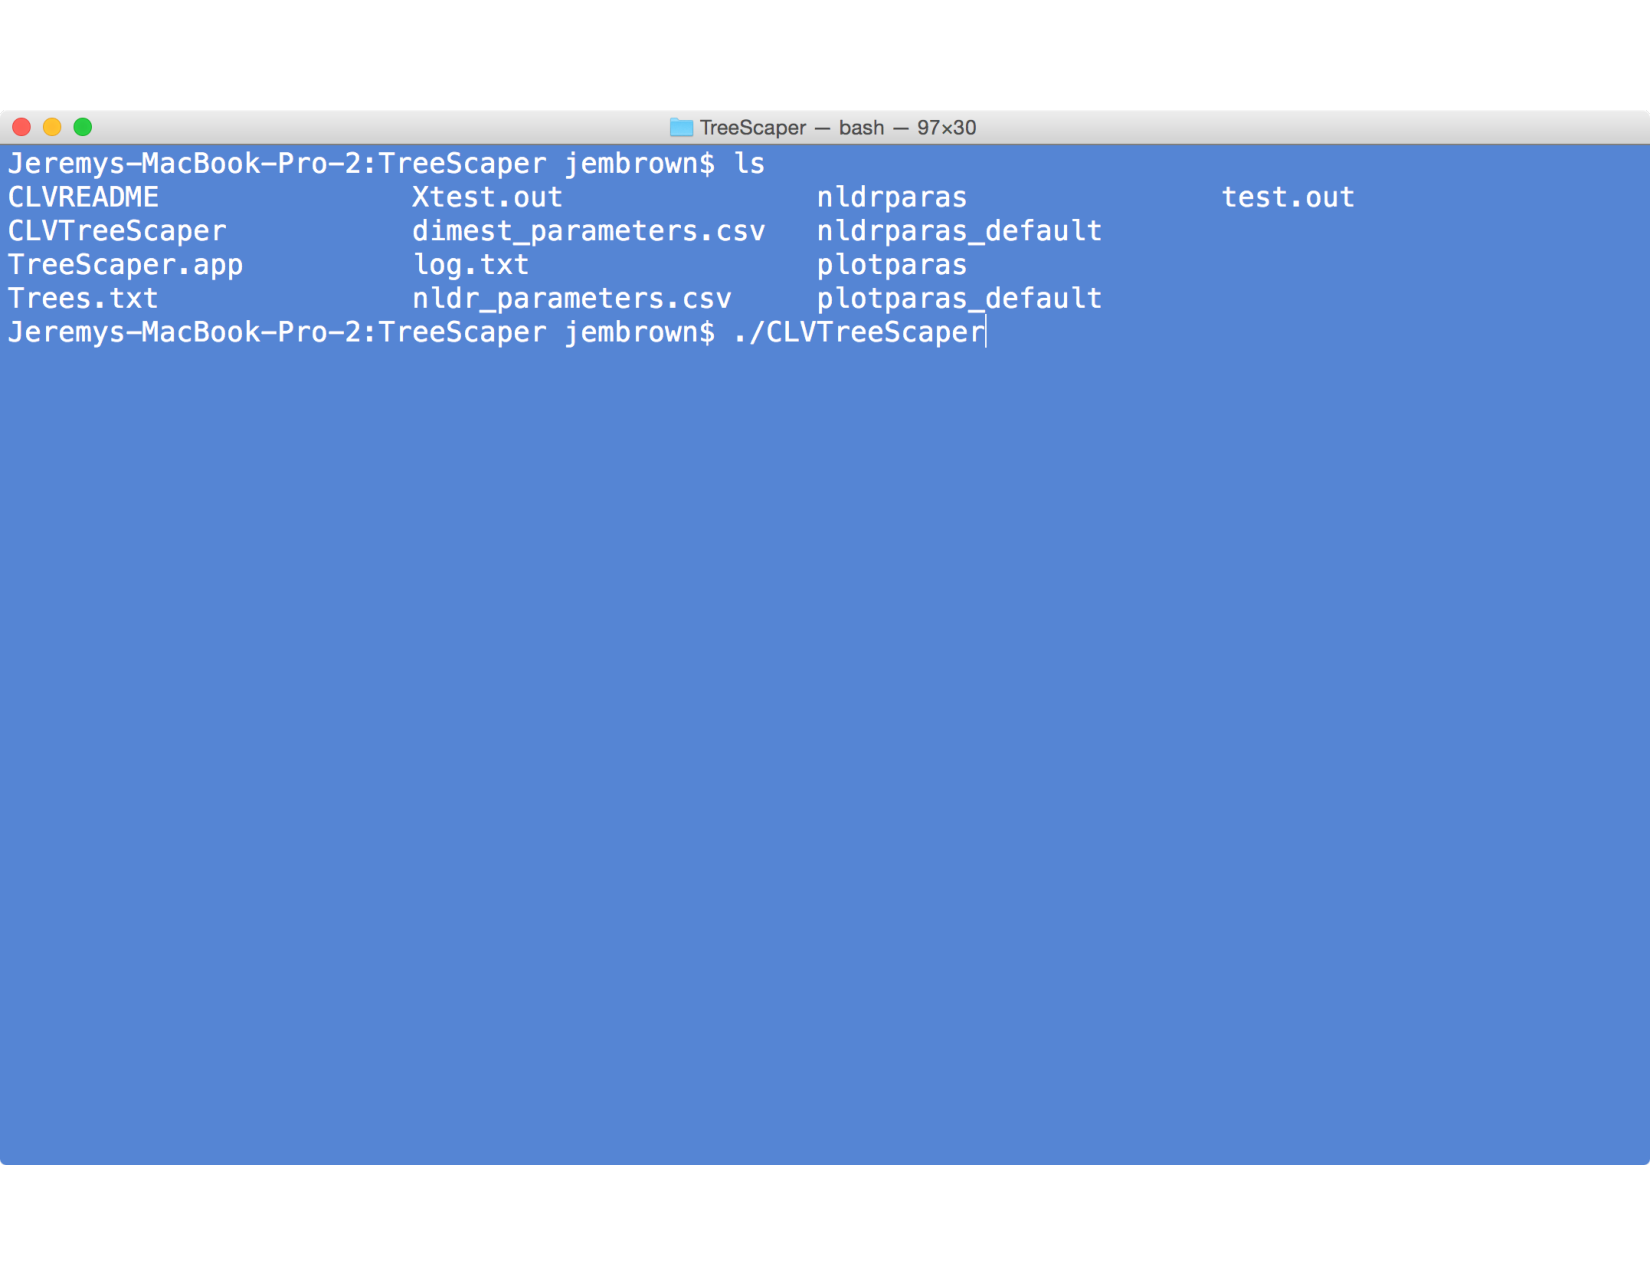
\includegraphics[scale=0.4]{imagesForManual/CLVTreeScaper.pdf}
%\caption{}\label{fig17}
\end{figure}

There are three general run modes for the command-line version of TreeScaper
(``CLVTreeScaper"). Using one of these three flags as the first command-line argument sets
the mode (e.g., CLVTreeScaper �trees).

\begin{enumerate}[{\bf (1)}]
\item {\bf -trees} 

In this mode, users can compute a majority rule/strict consensus tree, distance matrix,
bipartition matrix, covariance matrix, affinity matrix, or detect communities in an affinity or
covariance network. Relevant arguments include:
	\begin{description}
	\item[-f:] Provide the name of the file that contains the data
	
	\item[-ft:] The file type. Options are:
		\begin{description}
		\item[`Trees':] The file contains trees. The tree format can be either Newick or Nexus.
		\item[`Dist':] The file contains distance matrix which can be used to compute affinity matrix or communities.
		\item[`Cova':] The file contains covariance matrix which can be used to compute communities.
		\end{description}
	
	\item[-w:] Indicate whether trees are weighted. Options are:
		\begin{description}
		\item[`1':] weighted
		\item[`0':] unweighted
		\end{description}
	
	\item[-r:] Indicate whether trees are rooted. Options are:
		\begin{description}
		\item[`1':] rooted
		\item[`0':] unrooted
		\end{description}
	
	\item[-o:] This option is used to indicate what output the user is interested in. Options are:
		\begin{description}
			\item[`BipartMatrix']
			\item[`Consensus']
			\item[`Dist']
			\item[`Affinity']
			\item[`Covariance']
			\item[`Community']
		\end{description}
	\end{description}

\vspace{0.5cm}

When outputting a bipartition matrix (-o BipartMatrix):
	\begin{description}
	\item[-bfm:] Bipartition matrix output type. Options are: 
		\begin{description}
		\item[`list':] Output sparse matrix in the form (row, column, value)
		\item[`matrix':] Output as if it is a full matrix
		\end{description}
	\end{description}
	
\vspace{0.5cm}
		
When computing a majority-rule or strict consensus tree (-o Consensus), use the -if, -ct,
and/or -cfm flags:
	\begin{description}
	\item[-if:] The name of a list file. Consensus tree computations will only consider the trees indicated in the file.
	
	\item[-ct:] The type of consensus tree to be computed. Options are:
		\begin{description}
		\item[`Majority':] Majority consensus tree
		\item[`Strict':] Strict consensus tree
		\end{description}
	
	\item[-cfm:] Format of the consensus tree file. Options are:
		\begin{description}
		\item[`Newick']
		\item[`Nexus']
		\end{description}
	\end{description}

\vspace{0.5cm}
	
When computing a distance matrix (-o Dist):
	\begin{description}
	\item[-dm:] Indicates the distance metric. Options are:
		\begin{description}
		\item[`URF':] Unweighted Robinson-Foulds distance
		\item[`RF':] Weighted Robinson-Foulds distance
		\item[`Mat':] Matching distance
		\item[`SPR':] Subtree-Prune-Regraft
		\end{description}
	\end{description} 

\vspace{0.5cm}

When computing an affinity matrix (-o Affinity):
	\begin{description}
	\item[-dm:] Indicates the distance metric. Options are:
		\begin{description}
		\item[`URF']: Unweighted Robinson Foulds distance
		\item[`RF':] Weighted Robinson Foulds distance
		\item[`Mat':] Matching distance
		\item[`SPR':] Subtree-Prune and Regraft
		\end{description}
	
	\item[-am:] Indicates the distance to affinity transformation. Options are:
		\begin{description}
		\item[`Rec':] Reciprocal
		\item[`Exp':] Exponential
		\end{description}
	\end{description} 

\vspace{0.5cm}

When detecting communities (-o Community):
	\begin{description}
	\item[-t:] Target matrix used to compute communities. Options are:
		\begin{description}
		\item[`Affinity':] affinity matrix
		\item[`Covariance':] covariance matrix
		\end{description}
	
	\item[-cm:] Model used to compute communities. Options are:
		\begin{description}
		\item[`CNM':] Configuration Null Model
		\item[`CPM':] Constant Potts Model
		\item[`ERNM':] Erdos-R�nyi Null Model
		\item[`NNM':] No Null Model
		\end{description}
	
	\item[-lm:] Method of plateau detection. Options are:
		\begin{description}
		\item[`auto':] automatically choose lambdas and find plateaus
		\item[`manu':] specify intervals by users to find plateaus
		\end{description}
	\end{description}

\vspace{0.5cm}

The following flags are used to specify values of lambda for manual searches:
	\begin{description}
	\item[-lp:] Specify a fixed value of $\lambda^{+}$. Must be between 0 and 1. Used when -lpiv is zero (see below).
	
	\item[-lps, -lpe, -lpiv:] Starting, ending, and sampling intervals for $\lambda^{+}$. Used to explore a range of possible values for $\lambda^{+}$.
	
	\item[-ln:] Specify a fixed value of $\lambda^{-}$. Must be between $0$ and $1$. Used when -lniv is zero (see below).
	
	\item[-lns, -lne, -lniv:] Starting, ending, and sampling intervals for $\lambda^{-}$. Used to explore a range of possible values for $\lambda^{-}$. \\

{\it Note: Either $\lambda^{+}$ or $\lambda^{-}$ must be fixed, because plateau detection is undefined when both vary.} \\

	\item[-hf:] Frequency upper bound. A number between $0$ and $1$. Nodes with frequencies
above this value are ignored.

	\item[-lf:] Frequency lower bound. A number between $0$ and $1$. Nodes with frequencies
below this value are ignored.
	\end{description}

\vspace{0.5cm}

\ul{\bf Examples of command-line runs}
{\it Options specified by the are given inside braces. When specific alternatives are available, they
are separated by commas (e.g., \{option1,option2\}). When numbers can be specified anywhere in
a continuous range, the bounds of the range are separated by a dash (e.g., \{0-1\}).} \\


{\it Compute a Bipartition Matrix:} \\
./CLVTreeScaper -trees -f {trees.txt} -ft Trees -w {1,0} -r {1,0} -o BipartMatrix -bfm
\{list,matrix\} \\


{\it Compute a Consensus Tree:} \\
./CLVTreeScaper -trees -f \{trees.txt\} -ft Trees -w \{1,0\} -r \{1,0\} -o Consensus -if
IndicesFileName -ct \{Majority,Strict\} -cfm \{Newick,Nexus\} \\


{\it Compute Distance Matrix:} \\
./CLVTreeScaper -trees -f \{trees.txt\} -ft Trees -w \{1,0\} -r \{1,0\} -o Dist -dm \{URF,RF,Mat,SPR\} \\


{\it Compute Affinity Matrix:} \\
./CLVTreeScaper -trees -f \{trees.txt\} -ft Trees -w \{1,0\} -r \{1,0\} -o Affinity -dm \\
\{URF,RF,Mat,SPR\} -am \{Exp,Rec\} \\


{\it Compute Covariance Matrix:} \\
./CLVTreeScaper -trees -f \{trees.txt\} -ft Trees -w \{1,0\} -r \{1,0\} -o Covariance \\


{\it Compute Communities with $\lambda^{+}$ Fixed:} \\
./CLVTreeScaper -trees -f \{trees.txt\} -ft Trees -w \{1,0\} -r \{1,0\} -o Community -t \\
\{Affinity,Covariance\} -cm \{CNM,CPM,ERNM,NNM\} -lm manu -lp \{AnyNumber\} -lns \\
 \{AnyNumber\} -lne \{AnyNumber\} -lniv \{AnyNumber\} -hf \{0-1\} -lf \{0-1\} \\


{\it Compute Communities with $\lambda^{-}$ Fixed:} \\
./CLVTreeScaper -trees -f \{trees.txt\} -ft Trees -w \{1,0\} -r \{1,0\} -o Community -t \\
\{Affinity,Covariance\} -cm \{CNM,CPM,ERNM,NNM\} -lm manu -ln \{AnyNumber\} -lps \\
\{AnyNumber\} -lpe \{AnyNumber\} -lpiv \{AnyNumber\} -hf \{0-1\} -lf \{0-1\} \\


{\it Compute Communities with Automatically Chosen Lambdas:} \\
./CLVTreeScaper -trees -f \{trees.txt\} -ft Trees -w \{1,0\} -r \{1,0\} -o Community -t \\
\{Affinity/Covariance\} -cm \{CNM/CPM/ERNM/NNM\} -lm auto -hf \{0-1\} -lf \{0-1\} \\


{\it Load Distances and Compute Affinity Matrix:} \\
./CLVTreeScaper -trees -f \{dist.txt\} -ft Dist -o Affinity -am \{Exp,Rec\} \\


{\it Load Distances and Compute Affinity Communities Automatically:} \\
./CLVTreeScaper -trees -f \{dist.txt\} -ft Dist -o Community -t Affinity -am \{Exp,Rec\} -cm
\{CNM,CPM,ERNM,NNM\} -lm auto -hf \{0-1\} -lf \{0-1\} \\


{\it Load Covariances and Compute Communities using Automatic Search on Lambda:} \\
./CLVTreeScaper -trees -f \{cova.txt\} -ft Cova -o Community -cm \{CNM,CPM,ERNM,NNM\}
-lm auto -hf \{0-1\} -lf \{0-1\} \\ 


\item {\bf -nldr}

In this mode, users can project trees into lower dimensional space using non-linear
dimensionality reduction (NLDR). Relevant arguments include:
	\begin{description}
	\item[-f:] Name of the file containing distance data.
	
	\item[-t:] The type of distances contained in the file. Options are:
		\begin{description}
		\item[`DIS':] A lower triangle matrix of original distances
		\item[`COR':] Low-dimensional Euclidean coordinates (if already computed).
		\end{description}
	
	\item[-d:] The desired dimension of the Euclidean representation (usually 1, 2, or 3).
	
	\item[-c:] The chosen cost function. Options are:
		\begin{description}
		\item[`CLASSIC\_MDS�]
		\item[`KRUSKAL1�]
		\item[`NORMALIZED�]
		\item[`SAMMON�]
		\item[`CCA�]
		\end{description}
		
	\item[-a:] The chosen NLDR algorithm. Options are:
		\begin{description}
		\item[`LINEAR\_ITERATION�]
		\item[`MAJORIZATION�]
		\item[`GAUSS\_SEIDEL�]
		\item[`STOCHASTIC�]
		\end{description}
		
	\item[-i:] The method for generating initial Euclidean coordinates. Options are:
		\begin{description}
		\item[`RAND':] Randomly choose coordinates for each point.
		\item[`CLASSIC\_MDS':] Generate initial coordinates using classic multi-dimensional scaling (MDS).
		\end{description}
	
	\item[-o:] The suffix for output file names.
	
	\item[-s:] A random seed, if initial coordinates are generated randomly.
	\end{description}

\vspace{0.5 cm}	
	
\ul{\bf Example command:}\\
./CLVTreeScaper -nldr -f \{test.out\} -t \{DIS,COR\} -d \{1,2,3,�\} \\
-c \{CLASSIC\_MDS,KRUSKAL1,NORMALIZED,SAMMON,CCA\} \\
-a \{LINEAR\_ITERATION,MAJORIZATION,GAUSS\_SEIDEL,STOCHASTIC\} \\
-i \{RAND,CLASSIC\_MDS\} -o \{run1\} -s 1 \\


\item {\bf -dimest}

In this mode, users can estimate the intrinsic dimensionality of their data. This estimate can
help in deciding on an appropriate number of dimensions to use when performing NLDR
projections.
	\begin{description}
	\item[-f:] Name of the file containing distance data.
	
	\item[-i:] The type of distances contained in the file. Options are:
		\begin{description}
		\item[`DIS':] A lower triangle matrix of original distances
		\item[`COR':] Low-dimensional Euclidean coordinates (if already computed).
		\end{description}
	
	\item[-e:] The chosen estimator. Options are:
		\begin{description}
		\item[`CORR\_DIM':] Correlation dimension estimator
		\item[`NN\_DIM':] Nearest neighbor estimator
		\item[`MLE\_DIM':] Maximum likelihood estimator
		\end{description}
	\end{description}

\ul{\bf Example command:}\\
./CLVTreeScaper -dimest -f \{test.out\} -i \{DIS,COR\} -e \{CORR\_DIM,NN\_DIM,MLE\_DIM\} \\
\end{enumerate}

%%%%%%%%%%%%%%%%%%%%%%%%%%%%%%%%%%%%%%%%%%%%%%%%%%%
% APPENDIX (COMMUNITY DETECTION MODELS)
%%%%%%%%%%%%%%%%%%%%%%%%%%%%%%%%%%%%%%%%%%%%%%%%%%%
\newpage
\appendix
\section{COMMUNITY DETECTION MODELS}\label{appendix:CDModels}

Community detection includes a broad class of methods that attempt to find structure in
networks, by identifying groups of nodes that are more densely or tightly connected to each
other than they are to other nodes in the network {\color{red}\bf (REFERENCE NEEDED: (Newman 2010))}. These methods do not
require the number and size of groups (known as communities) to be identified in advance,
in contrast to graph partitioning approaches. Each of the community detection methods
implemented in TreeScaper employ a quantity known as the Hamiltonian ($\mathcal{H}$). Roughly
analogous to the use of this term in quantum mechanics, the Hamiltonian represents the
energy imposed by a given community structure. The structure with the minimum energy
represents the most natural division of nodes. Below we provide definitions of $\mathcal{H}$ for each of the methods in TreeScaper, as well as some explanation of how these definitions influence the
detected communities, in order to help users efficiently explore parameter space and properly
interpret model output. We also direct those interested to more in-depth explanations of
these methods in papers by ~\citep{Fortunato:2010,RB:2006,RAK:2007,TVDN:2011}. \\

%%%%%%%%%%%%%%%%%%%%%%%%%%%%%%%%%%%%%%%%%%%%%%%%%%%
% No Null Model
\subsection{No Null Model}\label{appendix:NoNullModel}
In the first case, which we term No Null Model (NNM, also known as the label propagation
method), $\mathcal{H}$ is defined for the set of all communities, $\{\sigma\}$, and is given by
\begin{equation}\label{eq:NoNullModel}
\mathcal{H}(\{\sigma\}) = - \displaystyle\sum_{i,j} A_{i,j} \delta(\sigma_{i}, \sigma{j}),
\end{equation}
where the sum is over all nodes $i$ and $j$, $A_{i,j}$ is the adjacency between nodes $i$ and $j$ (i.e., is there exists an edge connecting nodes $i$ and $j$), and $\sigma_{i}$ is the community to which bipartition $i$ belongs. $\delta(?_{i}, \sigma_{j})$ is defined as $1$ when $i$ and $j$ are in the same community, and $0$ otherwise. The NNM contains no tunable parameters and is generally of the least interest, since its Hamiltonian has only one global optimum with all nodes in a single community. However, local optima could be of some interest. \\


One way to refine our approach to community detection beyond the NNM involves first
defining an expectation for structure based on a stochastic model of network construction. In
these cases, the existence of communities can be revealed by comparison between the actual
density of edges in a subgraph and the density one would expect to have in the null subgraph
without community structure. The expected edge density depends on the chosen null model.
The two following methods are based on different choices of null model. \\


%%%%%%%%%%%%%%%%%%%%%%%%%%%%%%%%%%%%%%%%%%%%%%%%%%%
% Erdos-Renyi Model
\subsection{Erd\'{o}s-R\'{e}nyi Model}\label{appendix:ERModel}

For the Erd\'{o}s-R\'{e}nyi Model (ERM), $\mathcal{H}$ is given by
\begin{equation}\label{eq:ERModel1}
\mathcal{H}(\{\sigma\}) = - \displaystyle\sum_{i,j} \left[A_{i,j} -c^{2}\left(p_{i,j}^{+}\lambda^{+} - p_{i,j}^{-}\lambda^{-}\right)\right]\delta(\sigma_{i}, \sigma{j}),
\end{equation}
where $c$ is the size of the community in which $i$ and $j$ are placed, $p_{i,j}$ is the probability of a positive $(p_{i,j}^{+})$ or negative $(p_{i,j}^{-})$ edge between $i$ and $j$ in the null case, while $\lambda^{+}$ and $\lambda^{-}$ are tunable parameters. All other definitions are as Equation~\eqref{eq:NoNullModel} for the NNM. For Erd\'{o}s-R\'{e}nyi's random graph model, the probability of occurrence for any particular positive edge $(p_{i,j}^{+})$ is $m^{+} / n^{2}$, while the corresponding probability for any particular negative edge $(p_{i,j}^{-})$ is $m^{-} / n^{2}$, where $m^{+}$ is the sum of positive edge weights, $m^{-}$ is the sum of the absolute value of the negative edge weights, and $n$ is the number of nodes.\\


If community detection is performed on a bipartition covariance network and there are no
polytomies in the tree set, then for each bipartition, the sum of its covariances with all other
bipartitions equals zero. Correspondingly, the sum of the absolute value of the positive
covariances is equal to the sum of the absolute value of the negative covariances. In this case, Equation~\eqref{eq:ERModel1} simplifies to
\begin{equation}\label{eq:ERModel2}
\mathcal{H}(\{\sigma\}) = - \displaystyle\sum_{i,j} \left[A_{i,j} -c^{2}(p_{i,j}^{+}\left(\lambda^{+} - \lambda^{-}\right)\right]\delta(\sigma_{i}, \sigma{j}). \\
\end{equation}


For this model, changing the $\lambda$ tuning parameters affects the preferred community size by
adjusting the reward and penalty for including positive and negative edges, respectively, in a
community. In the simplified equation, if $\lambda^{+} > \lambda^{-}$, then small communities are preferred. If $\lambda^{-} > \lambda^{+}$, then large communities are preferred. \\


%%%%%%%%%%%%%%%%%%%%%%%%%%%%%%%%%%%%%%%%%%%%%%%%%%%
% Configuration Null Model
\subsection{Configuration Null Model}\label{appendix:CNModel}

For the Configuration Null Model (CNM), $\mathcal{H}$ is given by
\begin{equation}\label{eq:CNModel1}
\mathcal{H}(\{\sigma\}) = - \displaystyle\sum_{i,j} \left[A_{i,j} -  \left(\frac{k_{i}^{+} k_{j}^{+}}{m^{+}} \lambda^{+} - \frac{k_{i}^{-} k_{j}^{-}}{m^{-}} \lambda^{-}\right)\right]\delta(\sigma_{i}, \sigma{j}),
\end{equation}
where $k_{i}^{+}$ is the sum of all positive edges connecting nodes $i$, $k_{i}^{-}$ is the sum of the absolute value of all negative edges connecting to node $i$, $m^{+}$ is the sum of the positive edges in community $\sigma$, and $m^{-}$ is the sum of the absolute value of all negative edges in community $\sigma$. All of the other terms are as above. \\


If bipartition-covariance community detection is performed and there are no polytomies in
the tree set the above equation simplifies to:
\begin{equation}\label{eq:CNModel2}
\mathcal{H}(\{\sigma\}) = - \displaystyle\sum_{i,j} \left[A_{i,j} -  \frac{k_{i}^{+} k_{j}^{+}}{m^{+}} \left(\lambda^{+} - \lambda^{-}\right)\right]\delta(\sigma_{i}, \sigma{j}). \\
\end{equation}


As with ERM, changing the $\lambda$ tuning parameters affects the preferred community size by
adjusting the reward and penalty for including positive and negative edges, respectively. In
the simplified equation, if $\lambda^{+} > \lambda^{-}$, then communities are more likely to include negative edges. If $\lambda^{-} > \lambda^{+}$, then communities are less tolerant of negative edges and more strongly favor only positive edges. \\


%%%%%%%%%%%%%%%%%%%%%%%%%%%%%%%%%%%%%%%%%%%%%%%%%%%
% Constant Potts Model
\subsection{Constant Potts Model}\label{appendix:CPModel}

For the Constant Potts Model (CPM), $\mathcal{H}$ is given by
\begin{equation}\label{eq:CNModel2}
\mathcal{H}(\{\sigma\}) = - \displaystyle\sum_{i,j} \left[A_{i,j} -  c^{2}\left(\lambda^{+} - \lambda^{-}\right)\right]\delta(\sigma_{i}, \sigma{j}),
\end{equation}
where all terms are as above. As with the other models, changing the values of the ? tuning
parameters affects the preferred community size. If $\lambda^{+} > \lambda^{-}$, small communities are preferred. If $\lambda^{-} > \lambda^{+}$, large communities are preferred. \\


%%%%%%%%%%%%%%%%%%%%%%%%%%%%%%%%%%%%%%%%%%%%%%%%%%%
% REFERENCES
%%%%%%%%%%%%%%%%%%%%%%%%%%%%%%%%%%%%%%%%%%%%%%%%%%%
\newpage
%\nocite{*} % list uncited references (for development purposes only)
\bibliographystyle{apalike}	% use with package {cite}
\bibliography{TreeScaperManual_ref}	% use with package {cite}

\end{document}